\section{Runtime View}

To accomplish specific tasks of DREAM the components listed in \textit{Section 2.2} must interact with each other. To describe the type of interactions which occur between one another, in this section are presented the most relevant sequence diagrams.\\
All functionalities described by the following diagrams can be performed through both Web and Mobile application by the users. 


\def\fillandplacepagenumber{%
 \par\pagestyle{empty}%
\vbox to 0pt{\vss}\vfill
\vbox to 0pt{\baselineskip0pt
   \hbox to\linewidth{\hss}%
   \setlength{\footskip}{70pt}
   \baselineskip\footskip
   \hbox to\linewidth{%
     \hfil\thepage\hfil}\vss}}

\subsection{Farmer registers}

In this sequence diagram it is shown the process of registration attended by the farmer. It is supposed that the farmer has already selected is role in the registration form and the Web/Mobile Application shows him/her the related field.\\ 
After having switched from the\textit{login} page to the \textit{registration} one, he/she signs up filling in the registration form. Then, Web/MobileApplication checks that all the credentials inserted by the farmer are valid. Then, the registration request is sent from Web/MobileApplication to RegistrationService component which is in charge of retrieving position and mandal of the farmer (through GoogleMapsAPI) before storing his/her data persistently in the Database. Eventually, DatabaseAccess component is called to store the information in the Database. The result of the operation is propagated back to Web/Mobile Application, following in reverse order the same path as before. If the result is negative the registration should be repeated and an alert regarding registration failure is sent to the farmer. If the result is positive the farmer is redirected to a waiting page and the Web/mobile application calls RegistrationService component to send a confirmation email to the farmer. The function is propagated to EmailManager component which is in charge to check if the farmer has clicked on the confirmation link in the email within a certain time limit. The result of the operation is propagated back to Web/MobileApplication, following in reverse order the same path as before. If the result is negative an alert regarding confirmation failure is sent to the farmer and he/her has to request for the generation of a new confirmation email to repeat the process. If the result is positive the farmer is redirected to \textit{login} page.\\
The process of registration is different for the agronomist and the policy maker. In fact, the credentials to be inserted differ in particular in a unique id code which is checked calling an appropriate function to be propagated from Web/MobileApplication to RegistrationService. This component is in charge of verifying the id code calling TelanganaGovernmentService component. Eventually, the result of the operation is returned following in reverse order the same path as before and if it is false the filling operation must be repeated. 

\newpage
\begin{landscape}
\begin{figure}[h]
\vspace*{-2cm}
\noindent
\centering
\centerline{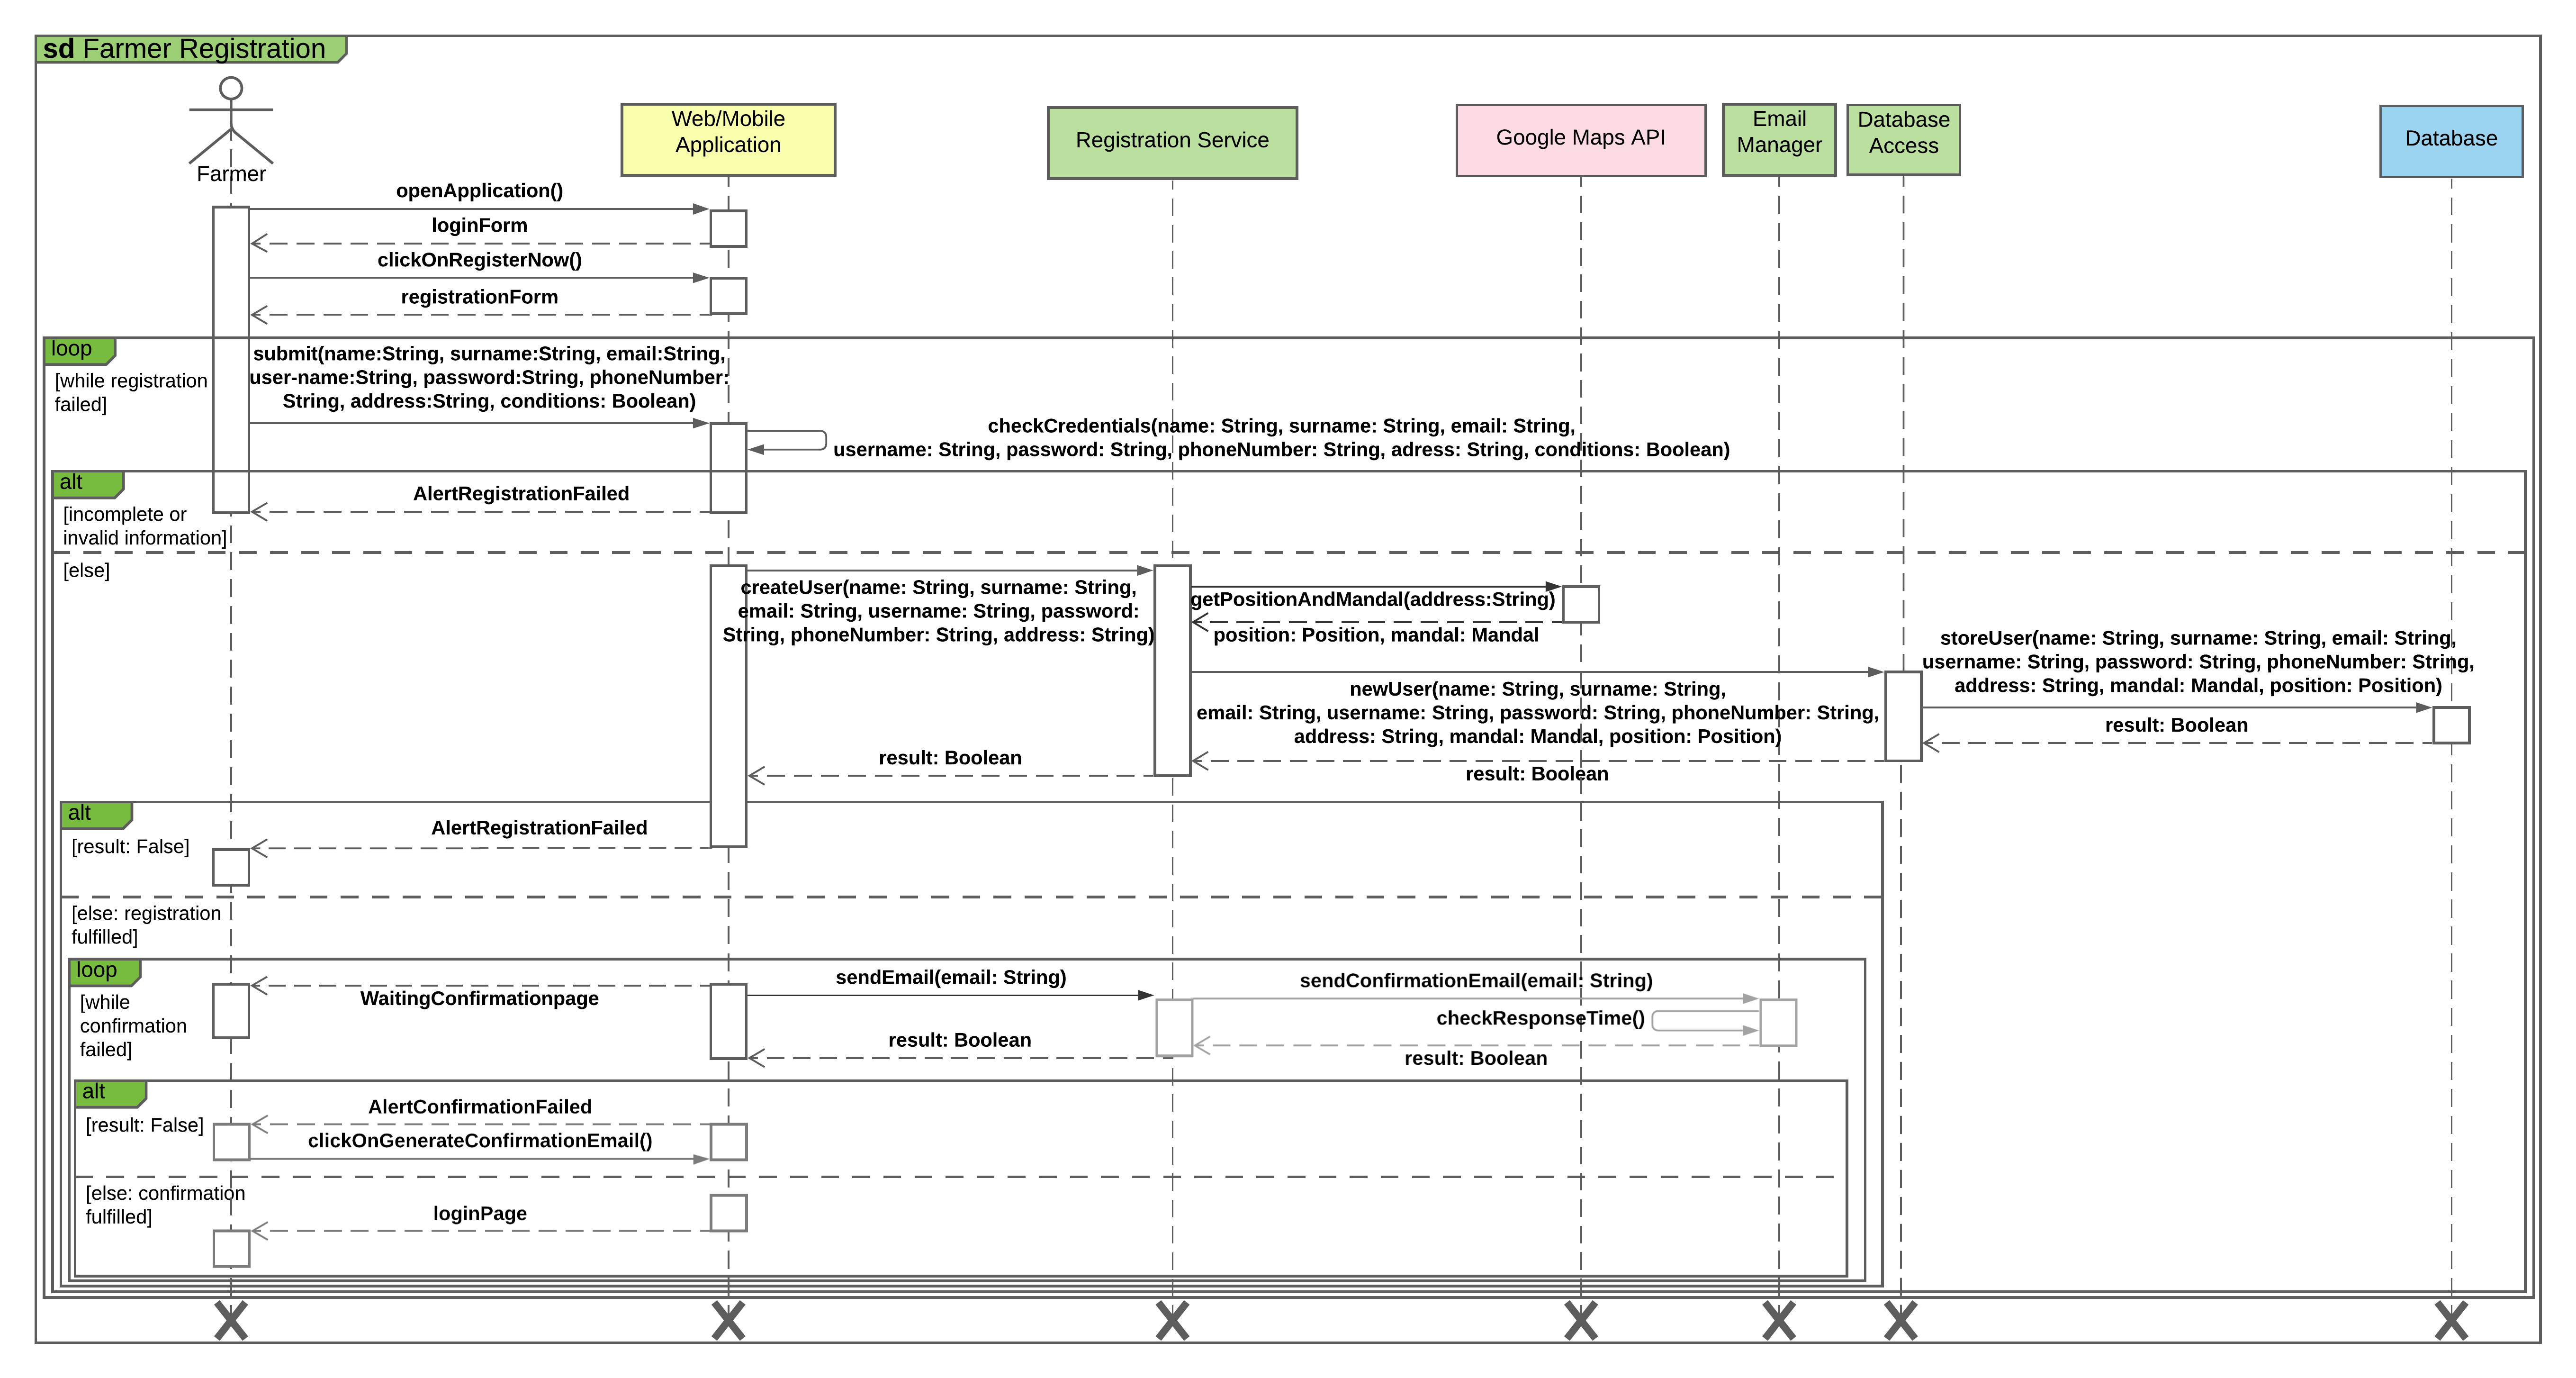
\includegraphics[scale= 0.108]{./Images/Sequence diagram/Farmer Registration Sequence Diagram.png}}
    \caption{Farmer Registration - Sequence Diagram}
    \vspace*{-12cm}
\end{figure}
\fillandplacepagenumber
\end{landscape}

\subsection{Farmer logs in}

This sequence diagram shows the login procedure executed by a farmer who is already registered.\\
After having opened DREAM application on his device, the farmer fills in the form with his username and password. The inserted credentials are checked by Web/MobileApplication, which controls whether one or both these two fields are missing. If it is the case, it shows to the farmer an alert regarding the login failure. If credentials are not missing, the AuthenticationService is called to check the validity of credentials and this component propagates the request to the DatabaseAccess that provides access to the Database, where all the users credentials are stored persistently. If a couple of username and password that matches the one inserted by the farmer is found, the login is successfully completed, otherwise an alert is shown and the operation must be repeated. This process is the same for all kind of users. \\
For the sake of completeness, in the sequence diagram it is shown also what is returned to the farmer who has successfully logged in. \\ 
The farmer must be able to visualize his/her \textit{homepage}, in which are reported weather conditions regarding his/her position and his/her next visit scheduled in the daily plan. For this reason a request to get weather conditions is propagated from Web/MobileApplication to WeatherConditionService which is able to retrieve weather and soil moisture from external APIs given the position of the user. The result of the operation is propagated to Web/MobileApplication. Then, the latter component send a request to VisitService. The request is propagated to DatabaseAccess to access the Database and retrieve all visits related to the farmer, which are returned eventually to VisitService, component that gets the next visit among them and returns it to Web/MobileApplication. Eventually, the \textit{homepage} is shown to the farmer. 

\newpage
\begin{landscape}
\begin{figure}[h]
\vspace*{-2cm}
\noindent
\centering
\centerline{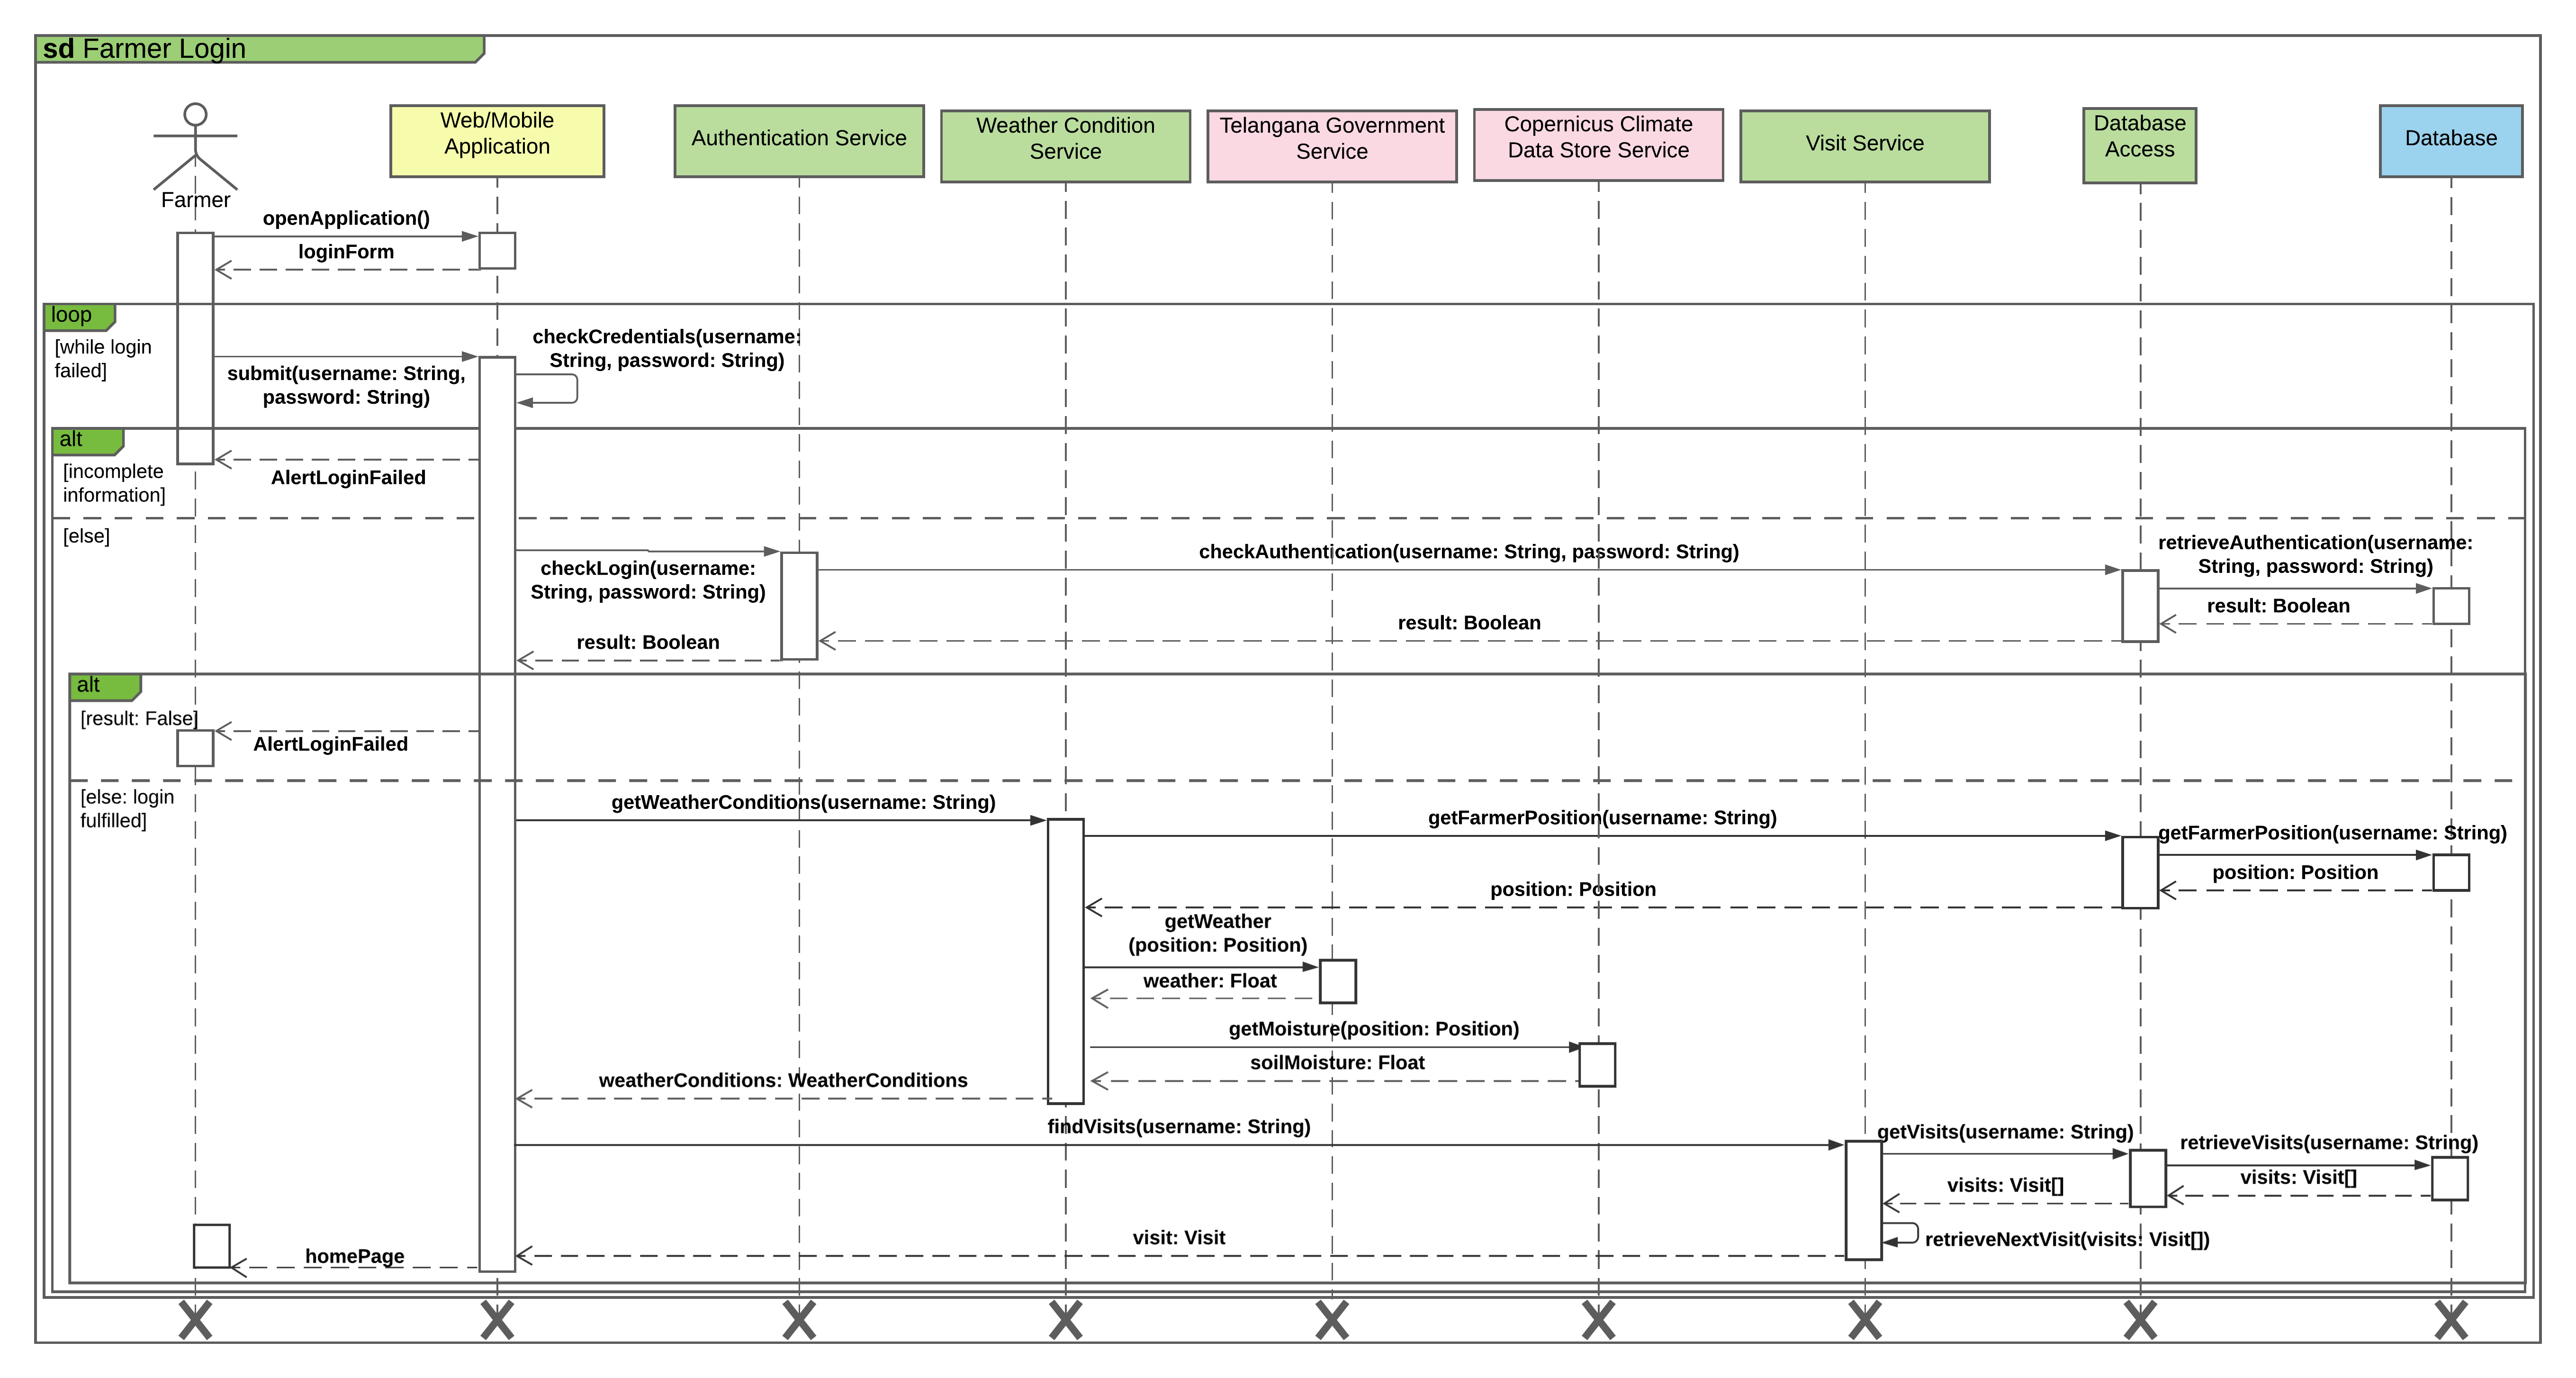
\includegraphics[scale= 0.108]{./Images/Sequence diagram/Farmer Login Sequence Diagram.png}}
    \caption{Farmer Login Sequence Diagram}
    \vspace*{-12cm}
\end{figure}
\fillandplacepagenumber
\end{landscape}

\subsection{Farmer inserts data about his/her production}

This sequence diagram shows the procedure of inserting data about production executed by a farmer who is already registered and logged in.\\
After having opened DREAM application on his device, the farmer clicks on \textit{Insert} icon in the homepage. Web/MobileApplication returns a form to be filled in. Once the farmer submits it Web/MobileApplication checks whether fields are missing or invalid. If it is the case, it shows an alert to the farmer. If it is not the case, the PerformanceService is called to compute the performance of the farmer.\\
Farmer's performance score is affected by weather conditions, for this reason it is necessary to retrieve farmer's position and his last performance date to define the time interval for which weather and soil moisture data must be retrieved. PerformanceService calls the DatabaseAccess. Database access provides access to the Database, where all the farmers' performances and positions are stored persistently. Farmer's last performance date and position are retrieved and returned eventually to PerformanceService.\\
The latter component is also able to get quantity of water consumed by the farmer calling TelanganaWaterIrrigationService. The result is returned back and a function is called by PerformanceService to add it to  the data inserted by the farmer. At this moment, two functions are called and propagated to two different external APIs (TelanganaGovernmentService and CopernicusClimateDataStoreService) to retrieve weather and soil moisture.\\ 
PerformanceService has now all necessary data to compute performance score, for which a proper function is called.\\
Eventually, farmer's performance is stored in the Database through a request which is propagated through DatabaseAccess to Database. A result is return following the same path. If it is false the process must be repeated. 

\newpage
\begin{landscape}
\begin{figure}[h]
\vspace*{-2cm}
\noindent
\centering
\centerline{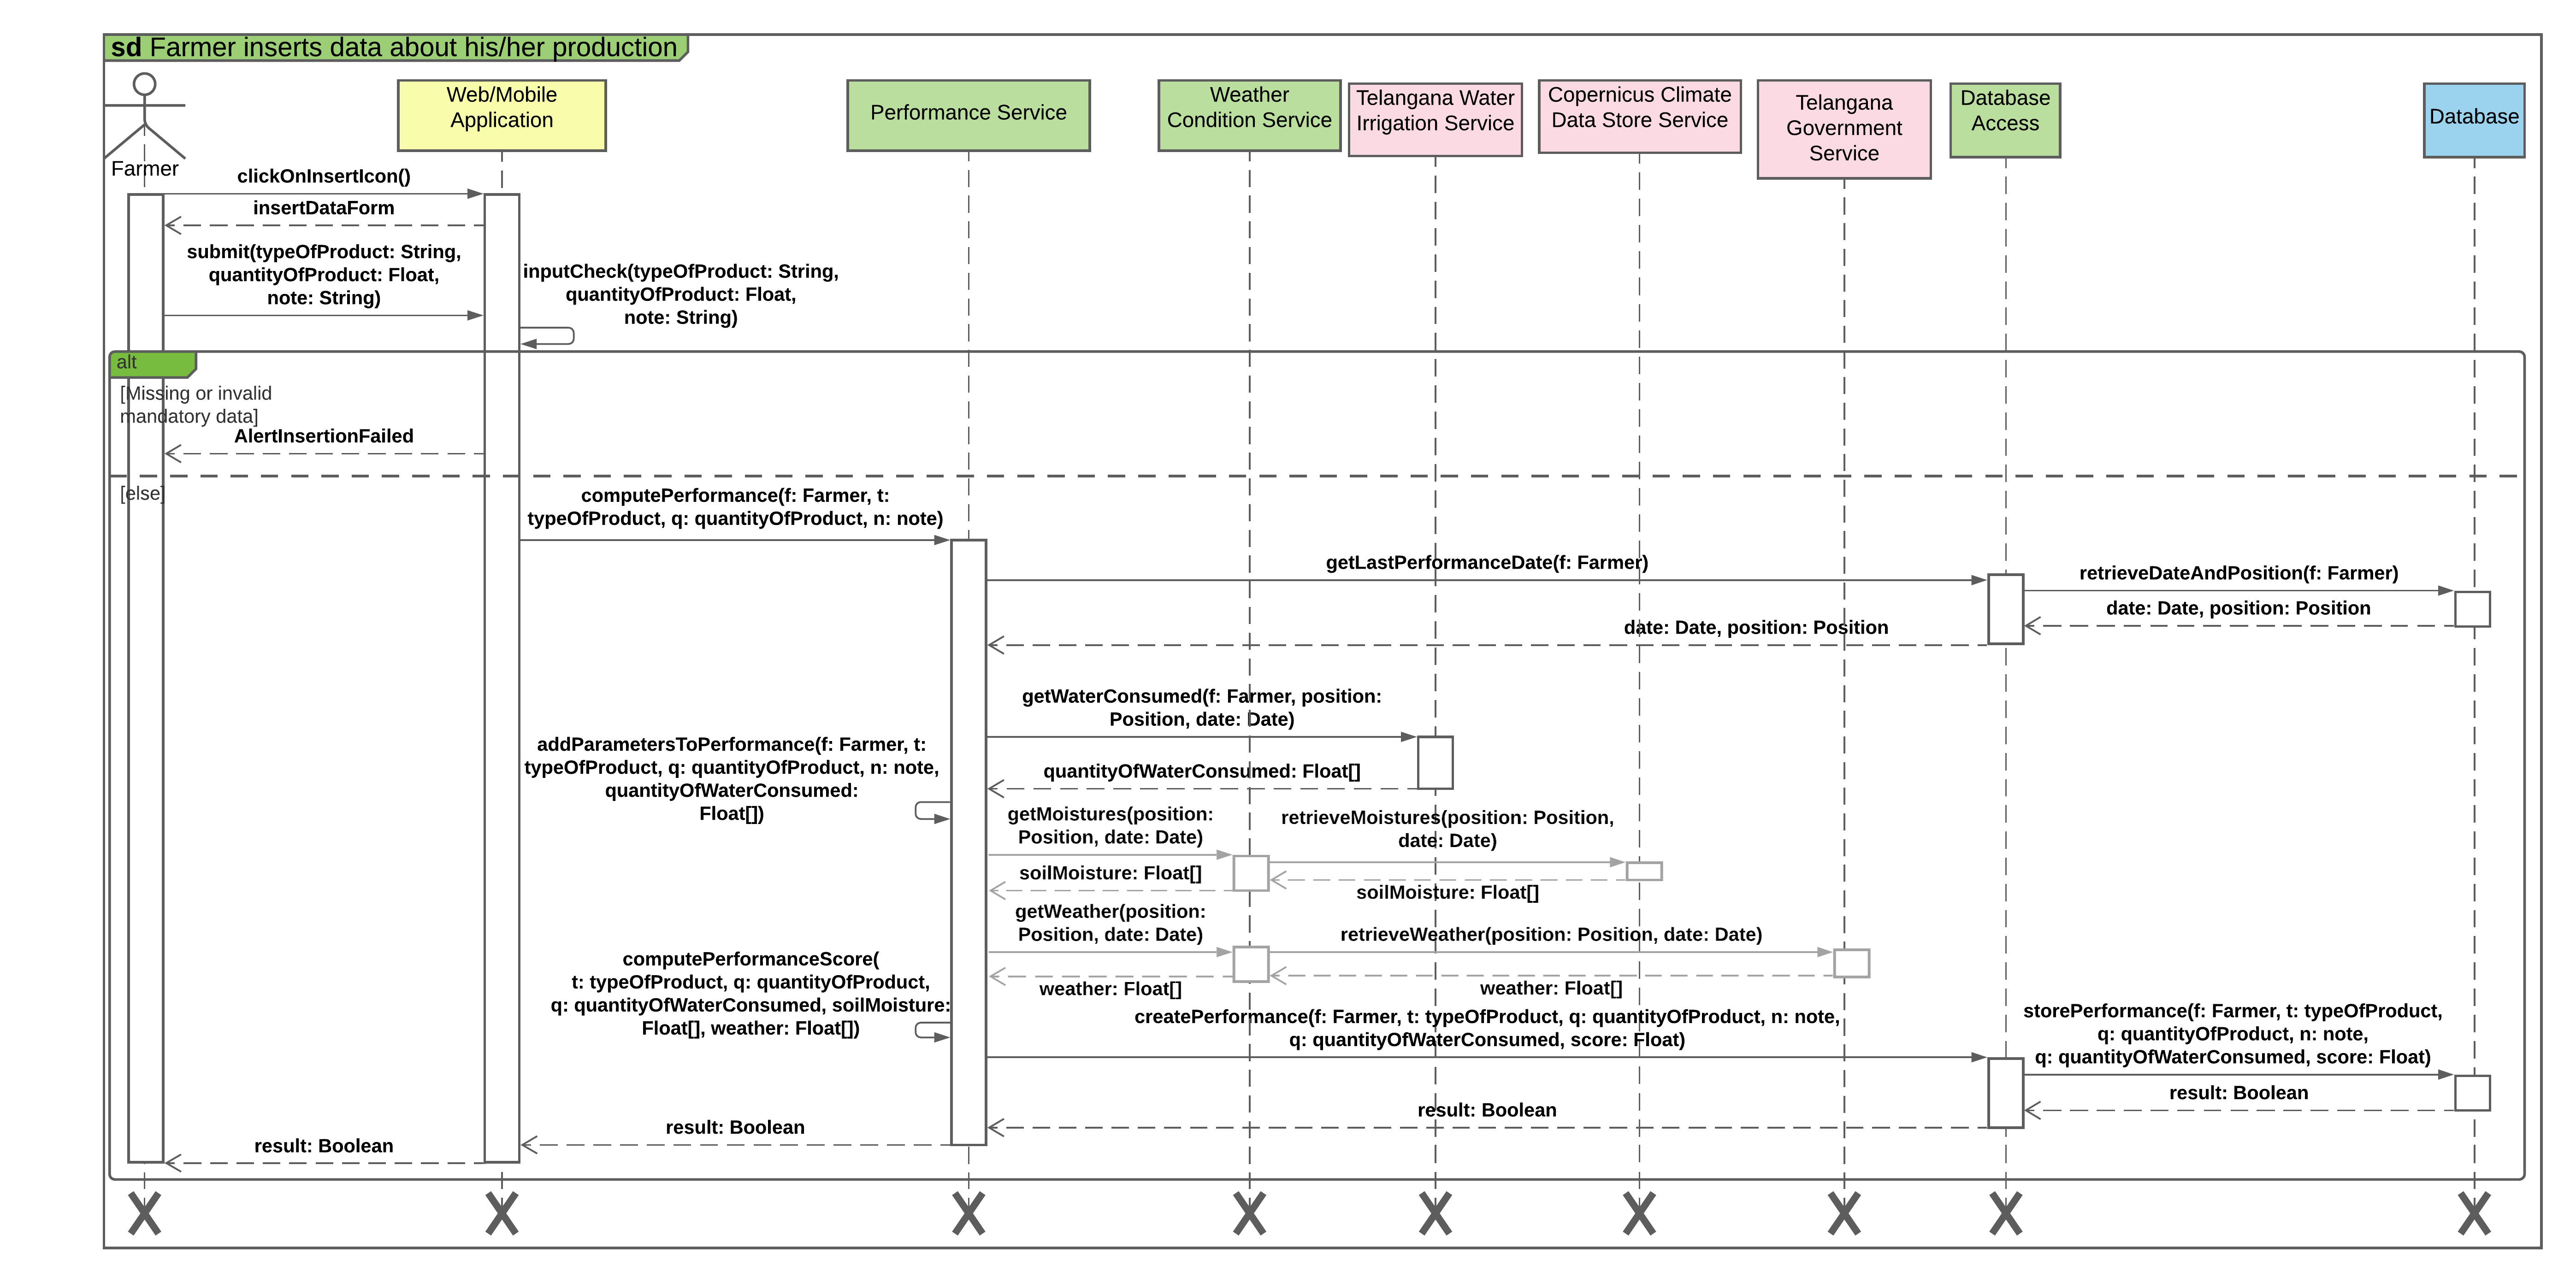
\includegraphics[scale= 0.108]{./Images/Sequence diagram/Farmer inserts data about his_her production.png}}
    \caption{Farmer inserts data about his/her production}
    \vspace*{-12cm}
\end{figure}
\fillandplacepagenumber
\end{landscape}

\subsection{DREAM sends suggestions to farmer}

This sequence diagram shows the procedure of DREAM sending periodic suggestions to a farmer who is already registered. Suggestions are computed by the system and affected by weather conditions regarding farmer's position and his/her last performance.\\
A request to compute suggestion is called by Web/MobileApplication and propagated to SuggestionService component which calls a function to get data needed to make the computation. For this reason the request is propagated through DatabaseAccess to Database. Farmer's last performance and position are eventually returned to SuggestionService. The latter component propagates two requests to get weather and soil moisture to WeatherConditionService, which is in charge to retrieve those data from external APIs (TelanganaGovernmentService and CopernicusClimateDataStoreService). Data are returned to SuggestionService which is now able to compute the suggestion calling a proper function. \\
Eventually, the suggestion is stored in the Database and is returned following the same path to Web/Mobile Application, which is able to send a notification to the farmer.

\newpage
\begin{landscape}
\begin{figure}[h]
\vspace*{-2cm}
\noindent
\centering
\centerline{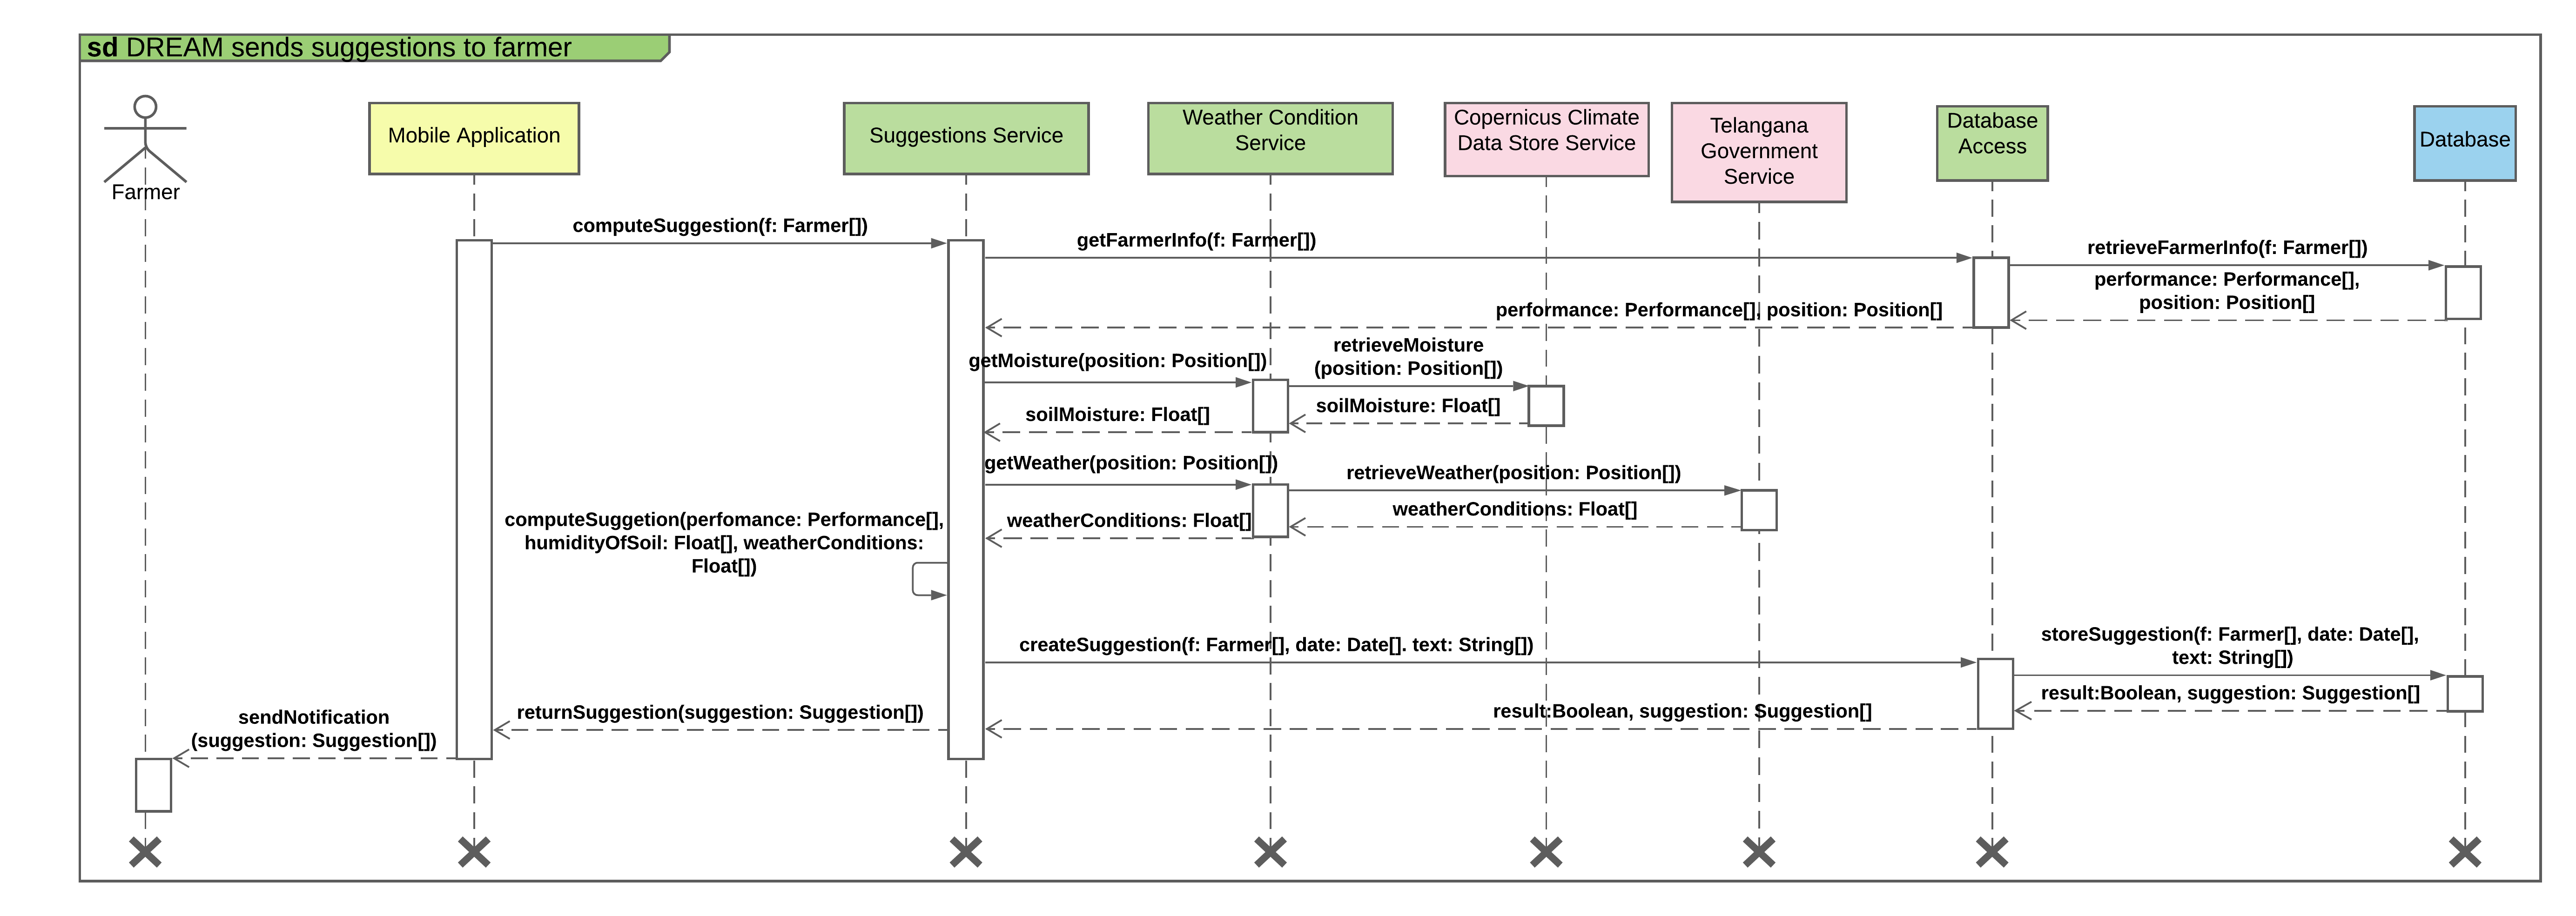
\includegraphics[scale= 0.108]{./Images/Sequence diagram/DREAM sends suggestions to farmer.png}}
    \caption{DREAM sends suggestions to farmer}
    \vspace*{-12cm}
\end{figure}
\fillandplacepagenumber
\end{landscape}

\subsection{Farmer searches for a thread in the discussion forum}

This sequence diagram shows the procedure of a farmer, already registered and logged in, searching for a thread on the discussion forum.\\
He/she clicks on \textit{discussion forum} icon. To return to the farmer the related page, Web/MobileApplication propagates a request to get all discussion forum's threads and related posts to DiscussionForumService which is able to retrieve them from the Database through DatabaseAccess.\\ 
Once the \textit{discussion forum} page is shown to the farmer, he/she clicks on \textit{search} icon and a form is returned by Web/MobileApplication. The farmer inserts the topic in the appropriated field and Web/MobileApplication calls a function to get all threads related to that topic. The request is propagated to DiscussionForumService which is in charge of finding those threads and their related posts. The result and found threads with related posts are returned to Web/MobileApplication following the same path. If result is false no thread was found and a message is sent to the user. If the result is true all found threads with related posts are shown to the farmer.

\newpage
\begin{landscape}
\begin{figure}[h]
\vspace*{-2cm}
\noindent
\centering
\centerline{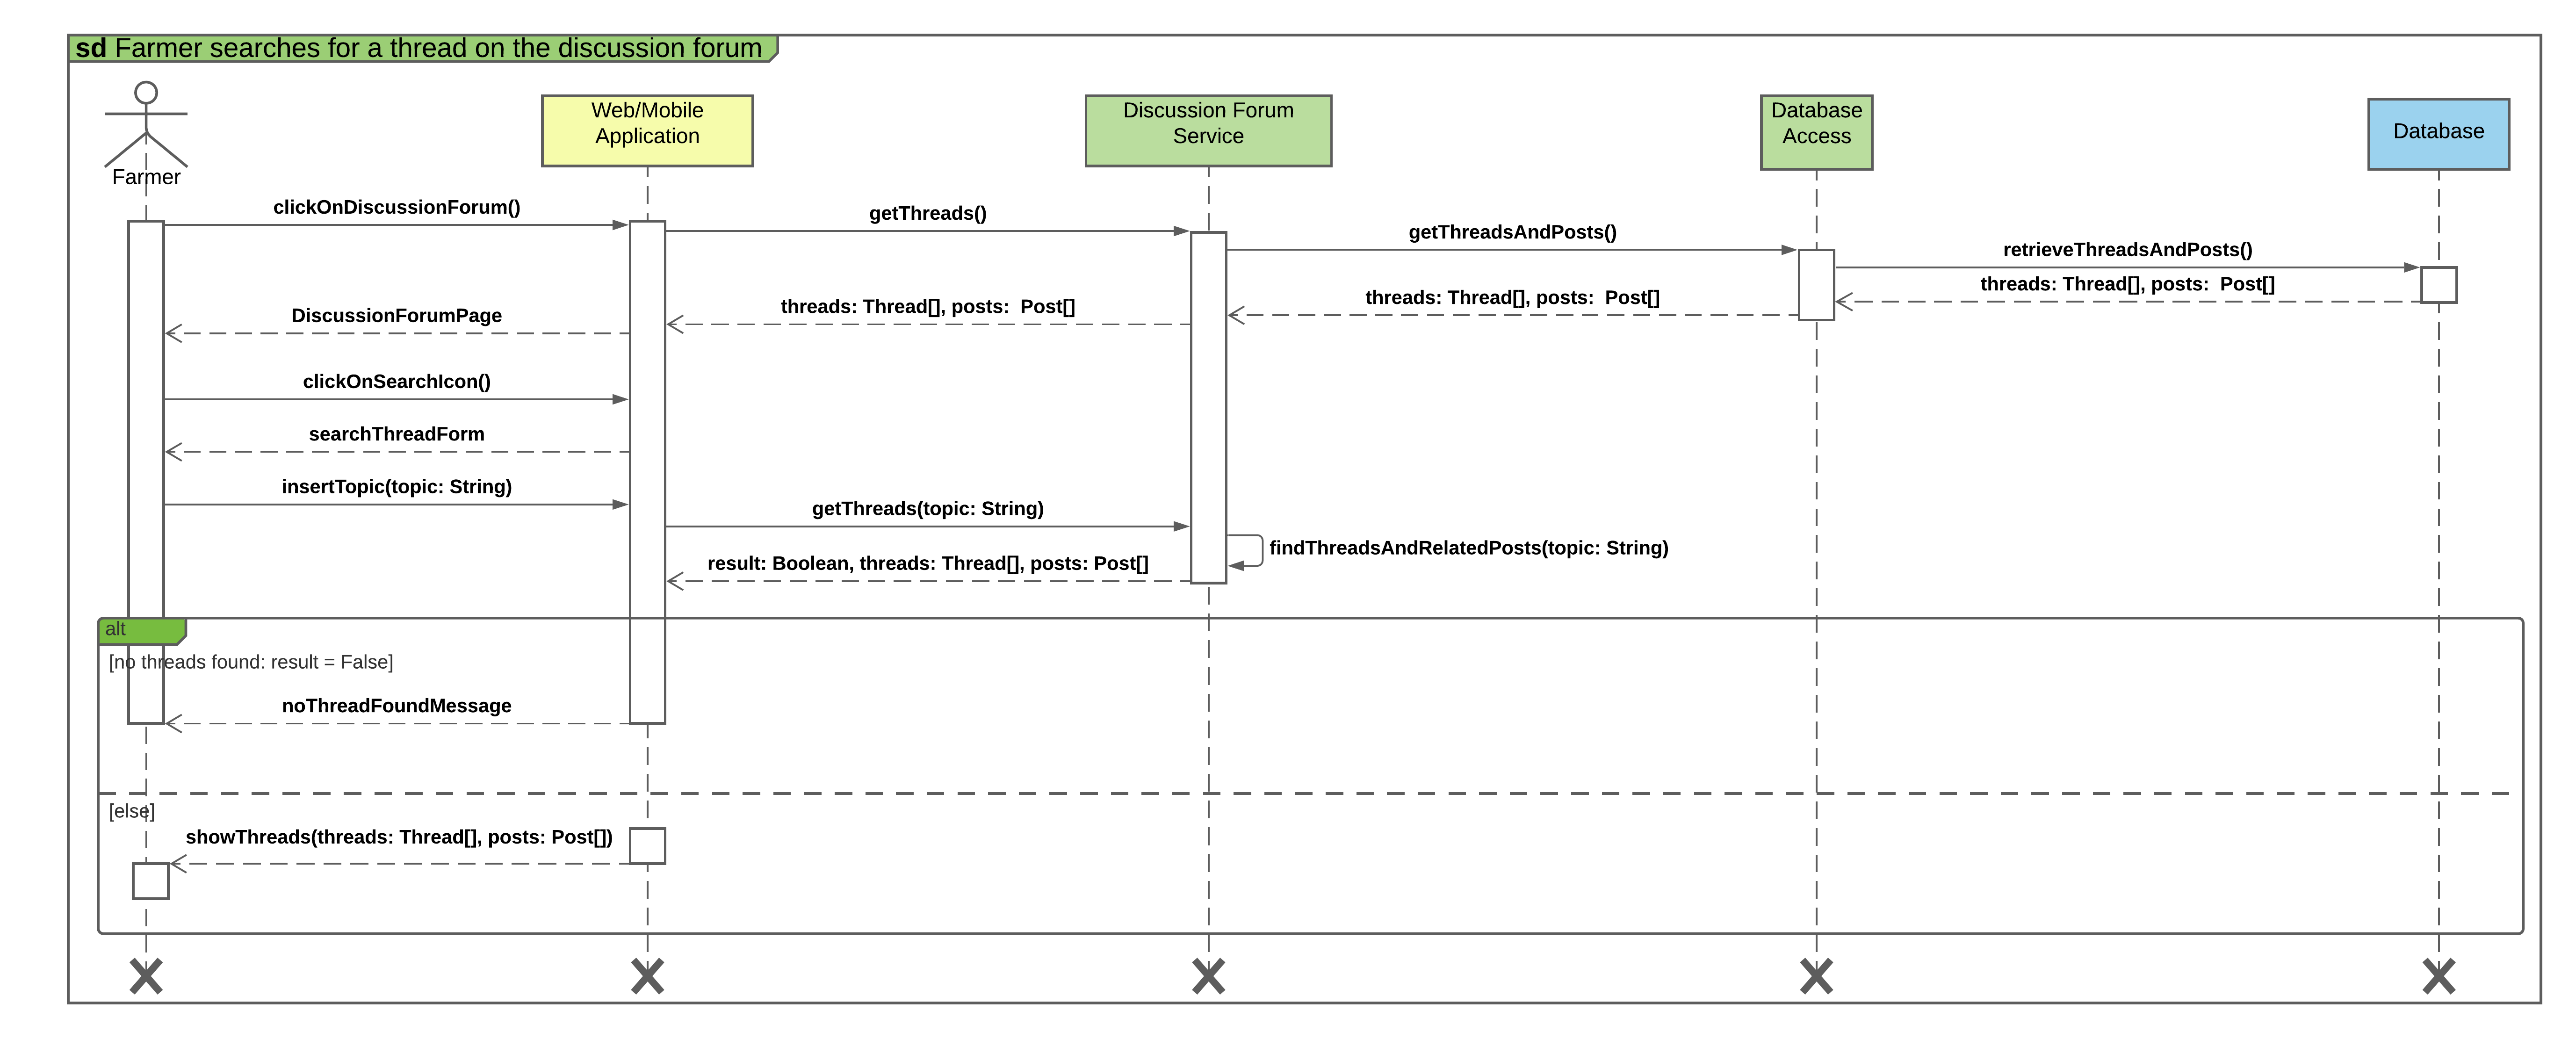
\includegraphics[scale= 0.108]{./Images/Sequence diagram/Farmer searches for a thread on the discussion forum.png}}
    \caption{Farmer searches for a thread in the discussion forum}
    \vspace*{-12cm}
\end{figure}
\fillandplacepagenumber
\end{landscape}

\subsection{Farmer creates a new thread in the discussion forum}

This sequence diagram shows the procedure of a farmer, already registered and logged in, opening a thread on the discussion forum.\\
He/she clicks on \textit{discussion forum} icon. To return to the farmer the related page, Web/MobileApplication propagates a request to get all discussion forum's threads and related posts to DiscussionForumService which is able to retrieve them from the Database through DatabaseAccess. 
Once the \textit{discussion forum} page is shown to the farmer, he/she clicks on \textit{new thread} button and a form is returned by Web/MobileApplication. The farmer inserts the topic and the text in the appropriated fields and Web/MobileApplication calls a function to store the new thread. The request is propagated to DiscussionForumService which is in charge of  adding additional information to the thread before propagating the request to Database through DatabaseAccess. The result is returned to Web/MobileApplication following the same path. If result is false the operation must be repeated.

\newpage
\begin{landscape}
\begin{figure}[h]
\vspace*{-2cm}
\noindent
\centering
\centerline{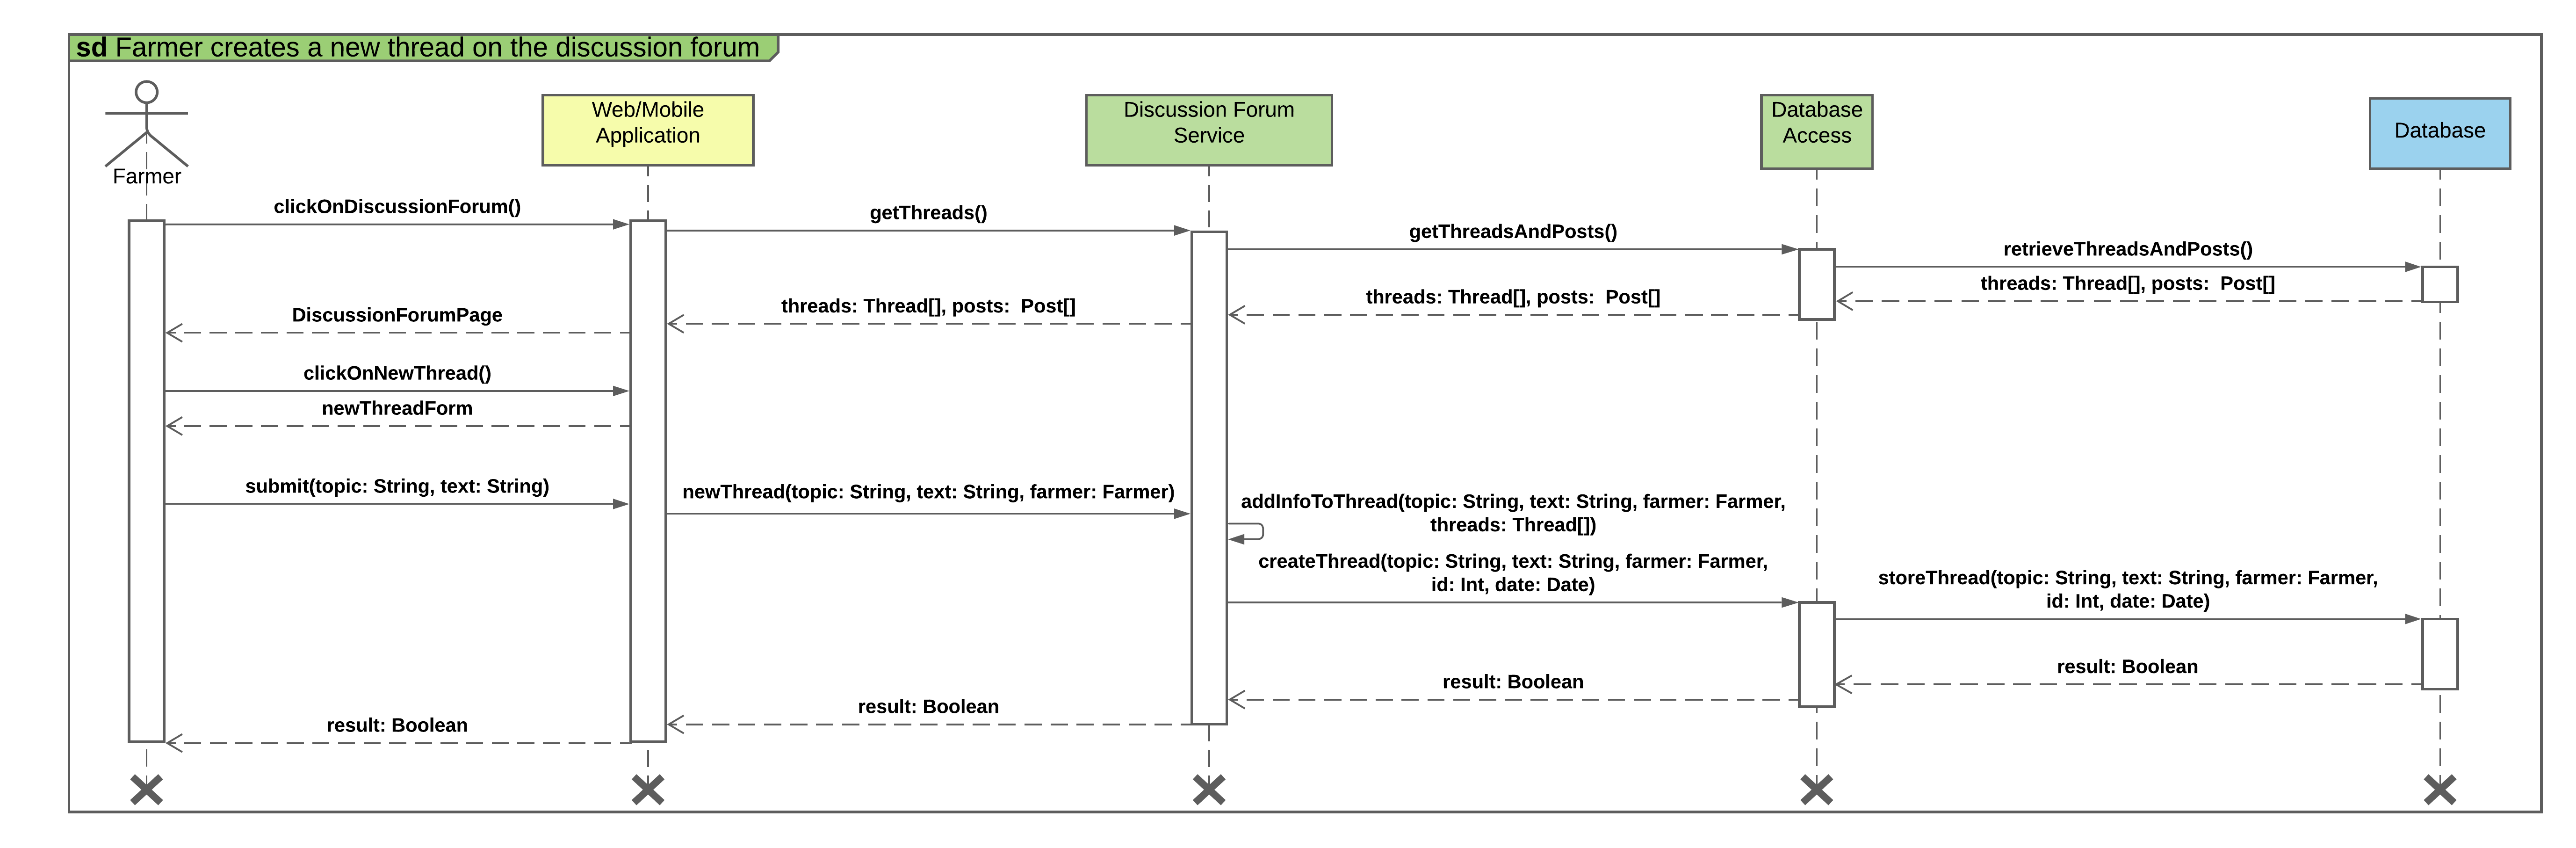
\includegraphics[scale= 0.108]{./Images/Sequence diagram/Farmer creates a new thread on the discussion forum.png}}
    \caption{Farmer creates a new thread in the discussion forum}
    \vspace*{-12cm}
\end{figure}
\fillandplacepagenumber
\end{landscape}

\subsection{Farmer replies in the discussion forum}

This sequence diagram shows the procedure of a farmer, already registered and logged in, replying on the discussion forum.\\
He/she clicks on \textit{discussion forum} icon. To return to the farmer the related page, Web/MobileApplication propagates a request to get all discussion forum's threads and related posts to DiscussionForumService which is able to retrieve them from the Database through DatabaseAccess. 
Once the \textit{discussion forum} page is shown to the farmer, he/she clicks on a thread whose details are returned by Web/MobileApplication after a function to find related posts is called. The farmer clicks on \textit{comment} button and a form is returned. He/she inserts the text of the post and Web/MobileApplication calls a function to store the new post. The request is propagated to DiscussionForumService which is in charge of  adding additional information to the post before propagating the request to Database through DatabaseAccess. The result is returned to Web/MobileApplication following the same path. If result is false the operation must be repeated. If the result is true the process is successfully completed and a message is sent to the farmer who created the post while a notification is sent to the one that has created the related thread. 

\newpage
\begin{landscape}
\begin{figure}[h]
\vspace*{-2cm}
\noindent
\centering
\centerline{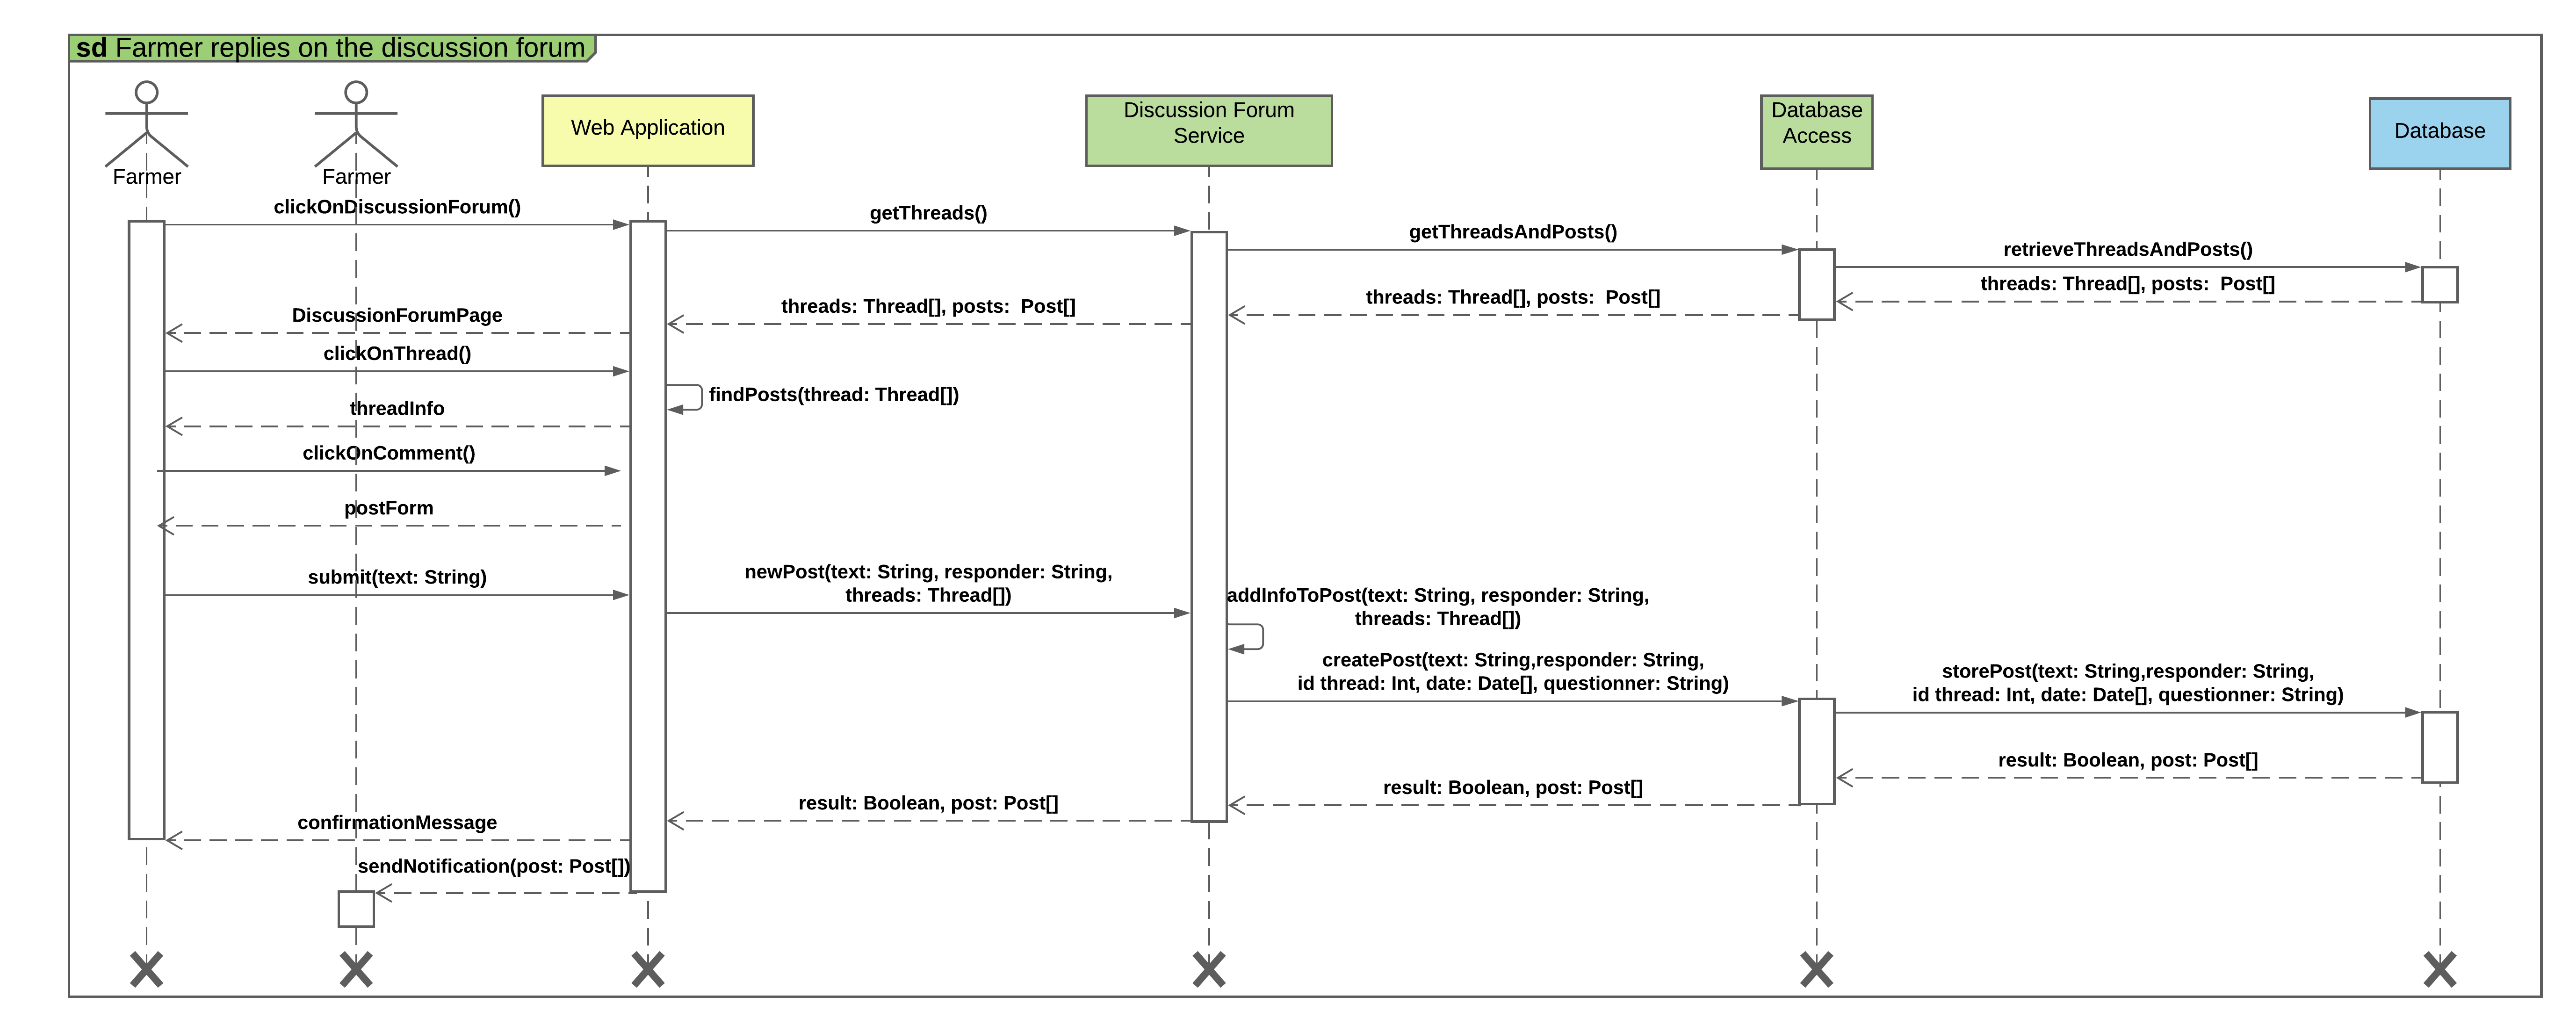
\includegraphics[scale= 0.108]{./Images/Sequence diagram/Farmer replies on the discussion forum.png}}
    \caption{Farmer replies on the discussion forum}
    \vspace*{-12cm}
\end{figure}
\fillandplacepagenumber
\end{landscape}

\subsection{Farmer creates a help request}

This sequence diagram shows the procedure of a farmer, already registered and logged in, creating a help request.\\
He/she clicks on \textit{help request} icon. To return to the farmer the related page, Web/MobileApplication propagates a request to get all help requests and related help responses related to the farmer to HelpRequestService which is able to retrieve them from the Database through DatabaseAccess. 
Once the \textit{help request} page is shown to the farmer, he/she clicks on \textit{create help request} button and a form is returned by Web/MobileApplication. The farmer inserts the text in the appropriated field and checks well performing farmers as recipient if he/she wants to. Web/MobileApplication calls a function to store the new thread. The request is propagated to HelpRequestService which is in charge of  adding additional information to the help request before returning the help request following the same path to show its details to the farmer. The help request is then stored in the Database. The result and the help request are returned to Web/MobileApplication following the same path. If result is false the operation must be repeated. If it is true a notification is always sent to the agronomist responsible of the mandal which the farmer is located in. If well performing farmers are also checked as recipient a function is called by PerformanceService to get well performing farmers given all farmers' performances. The farmers retrieved are returned to Web/MobileApplication which is now able to send them a notification about the new help request received. 

\newpage
\begin{landscape}
\begin{figure}[h]
\vspace*{-2cm}
\noindent
\centering
\centerline{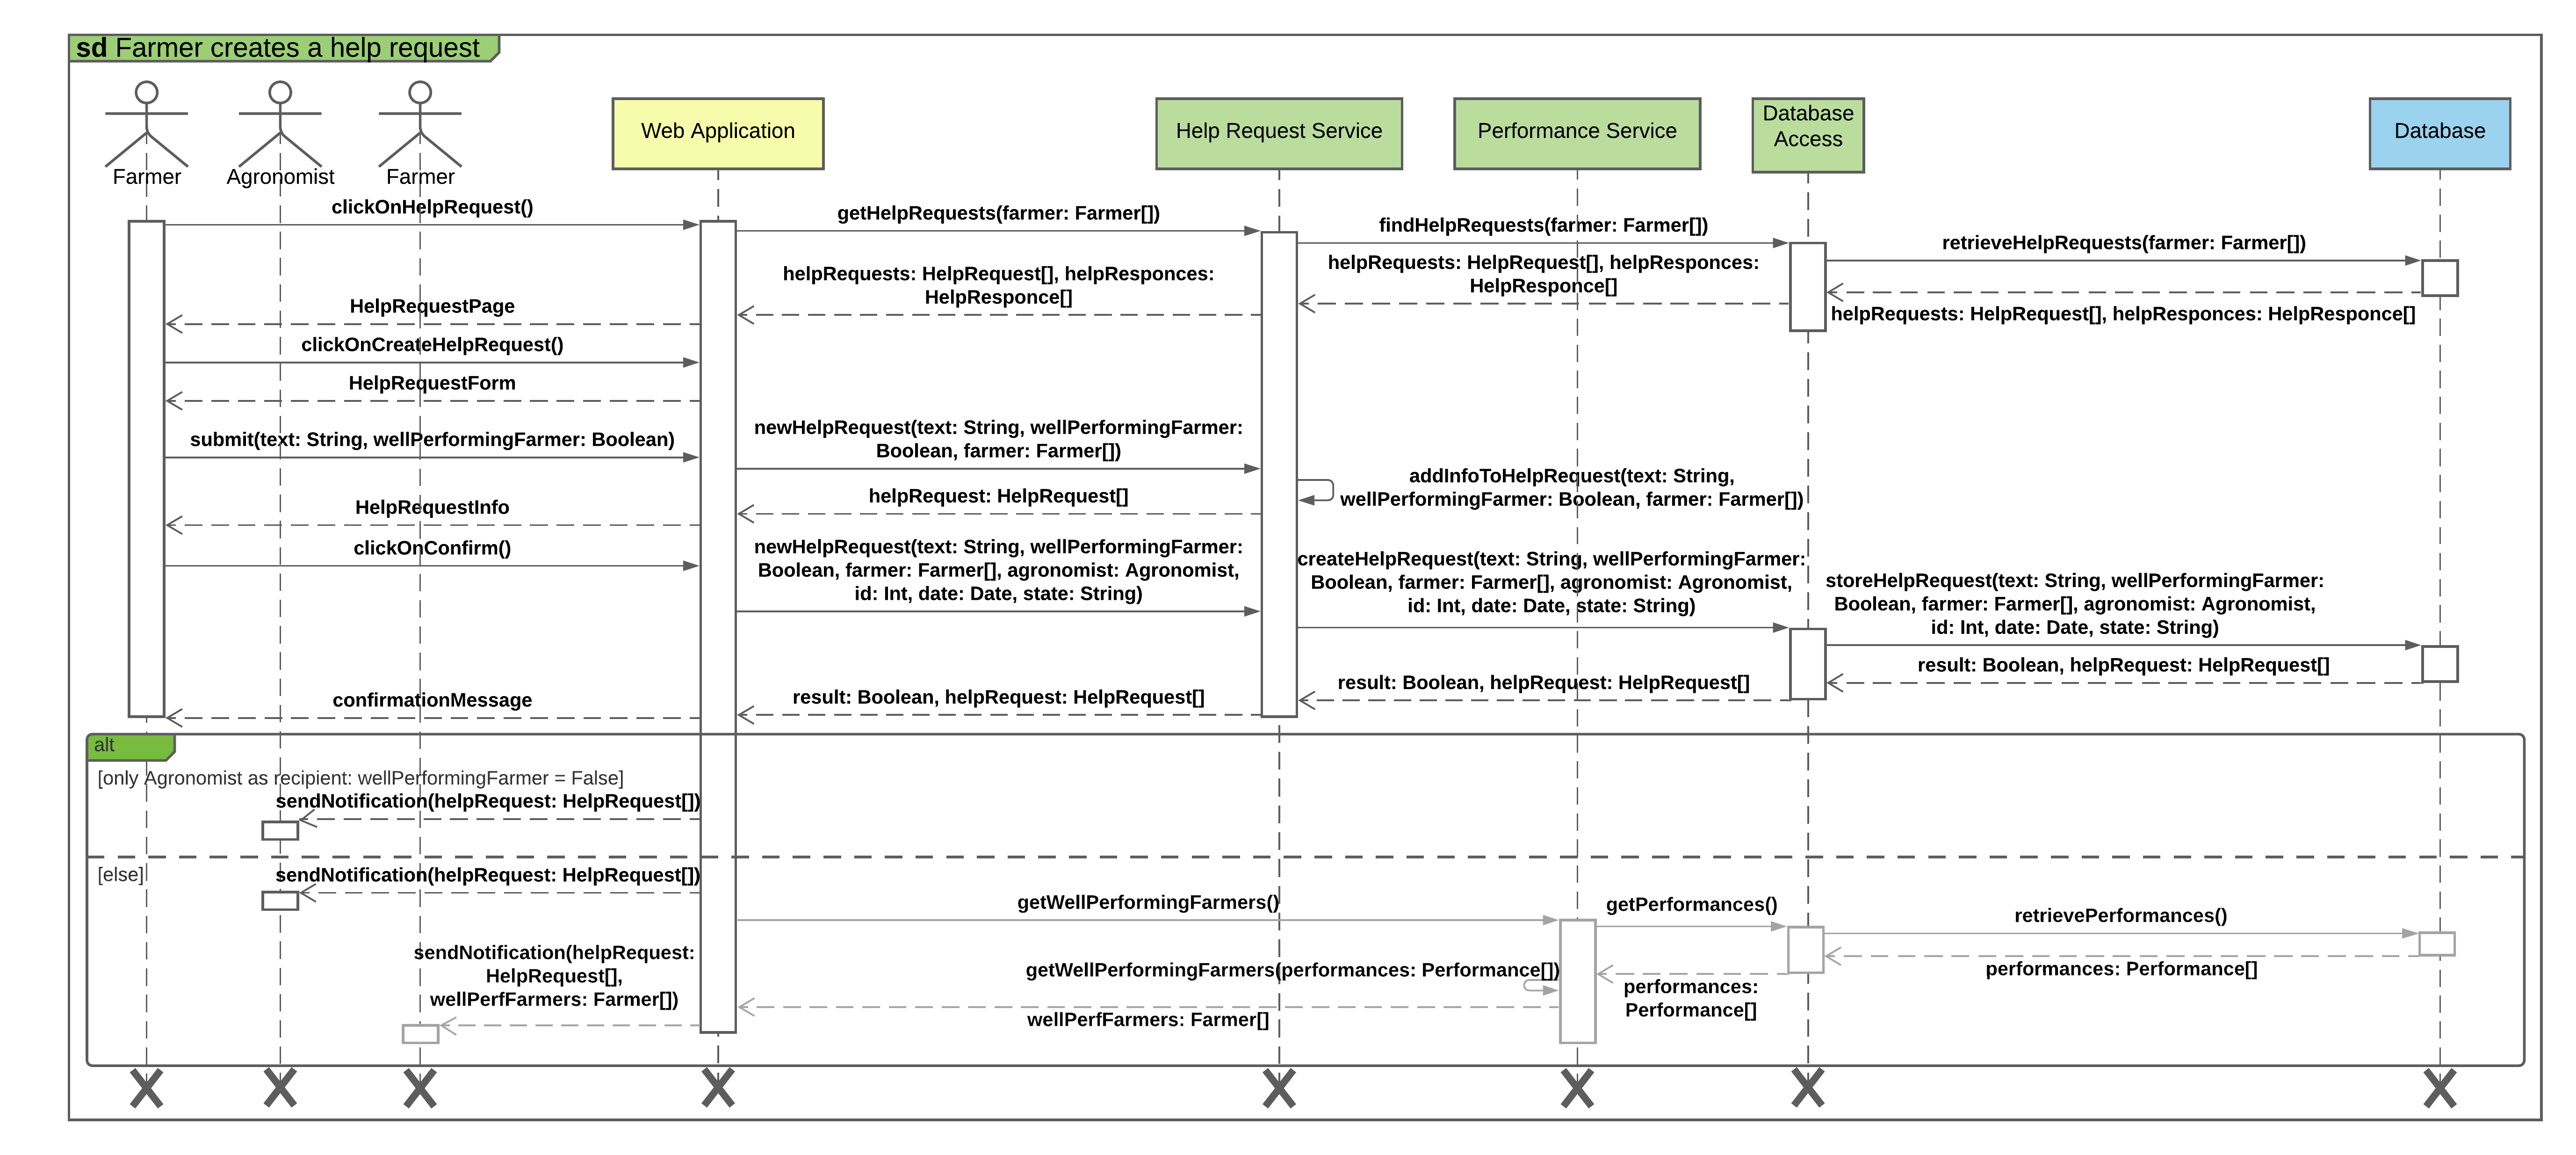
\includegraphics[scale= 0.108]{./Images/Sequence diagram/Farmer creates a help request.png}}
    \caption{Farmer creates a help request}
    \vspace*{-12cm}
\end{figure}
\fillandplacepagenumber
\end{landscape}

\subsection{Agronomist replies to a help request}

This sequence diagram shows the procedure of an agronomist, already registered and logged in, replying to a help request. The same functionality can be performed by a well performing farmer if he/she is checked as recipient in the help request.\\
The agronomist clicks on \textit{help request} icon. To return to the agronomist the related page, Web/MobileApplication propagates a request to get all help requests related to the agronomist to HelpResponseService which is able to retrieve them from the Database through DatabaseAccess. 
Once the \textit{help request} page is shown to the agronomist, he/she clicks on \textit{reply} button and a form is returned by Web/MobileApplication. The agronomist inserts the text in the appropriated field and Web/MobileApplication calls a function to store the new help response. The request is propagated to HelpResponseService which is in charge of  adding additional information to the help response. The help response is then stored in the Database. The result and the help response are returned to Web/MobileApplication following the same path. If result is false the operation must be repeated. If it is true a notification is sent to the farmer who made the help request and a confirmation message is sent to the agronomist.

\newpage
\begin{landscape}
\begin{figure}[h]
\vspace*{-2cm}
\noindent
\centering
\centerline{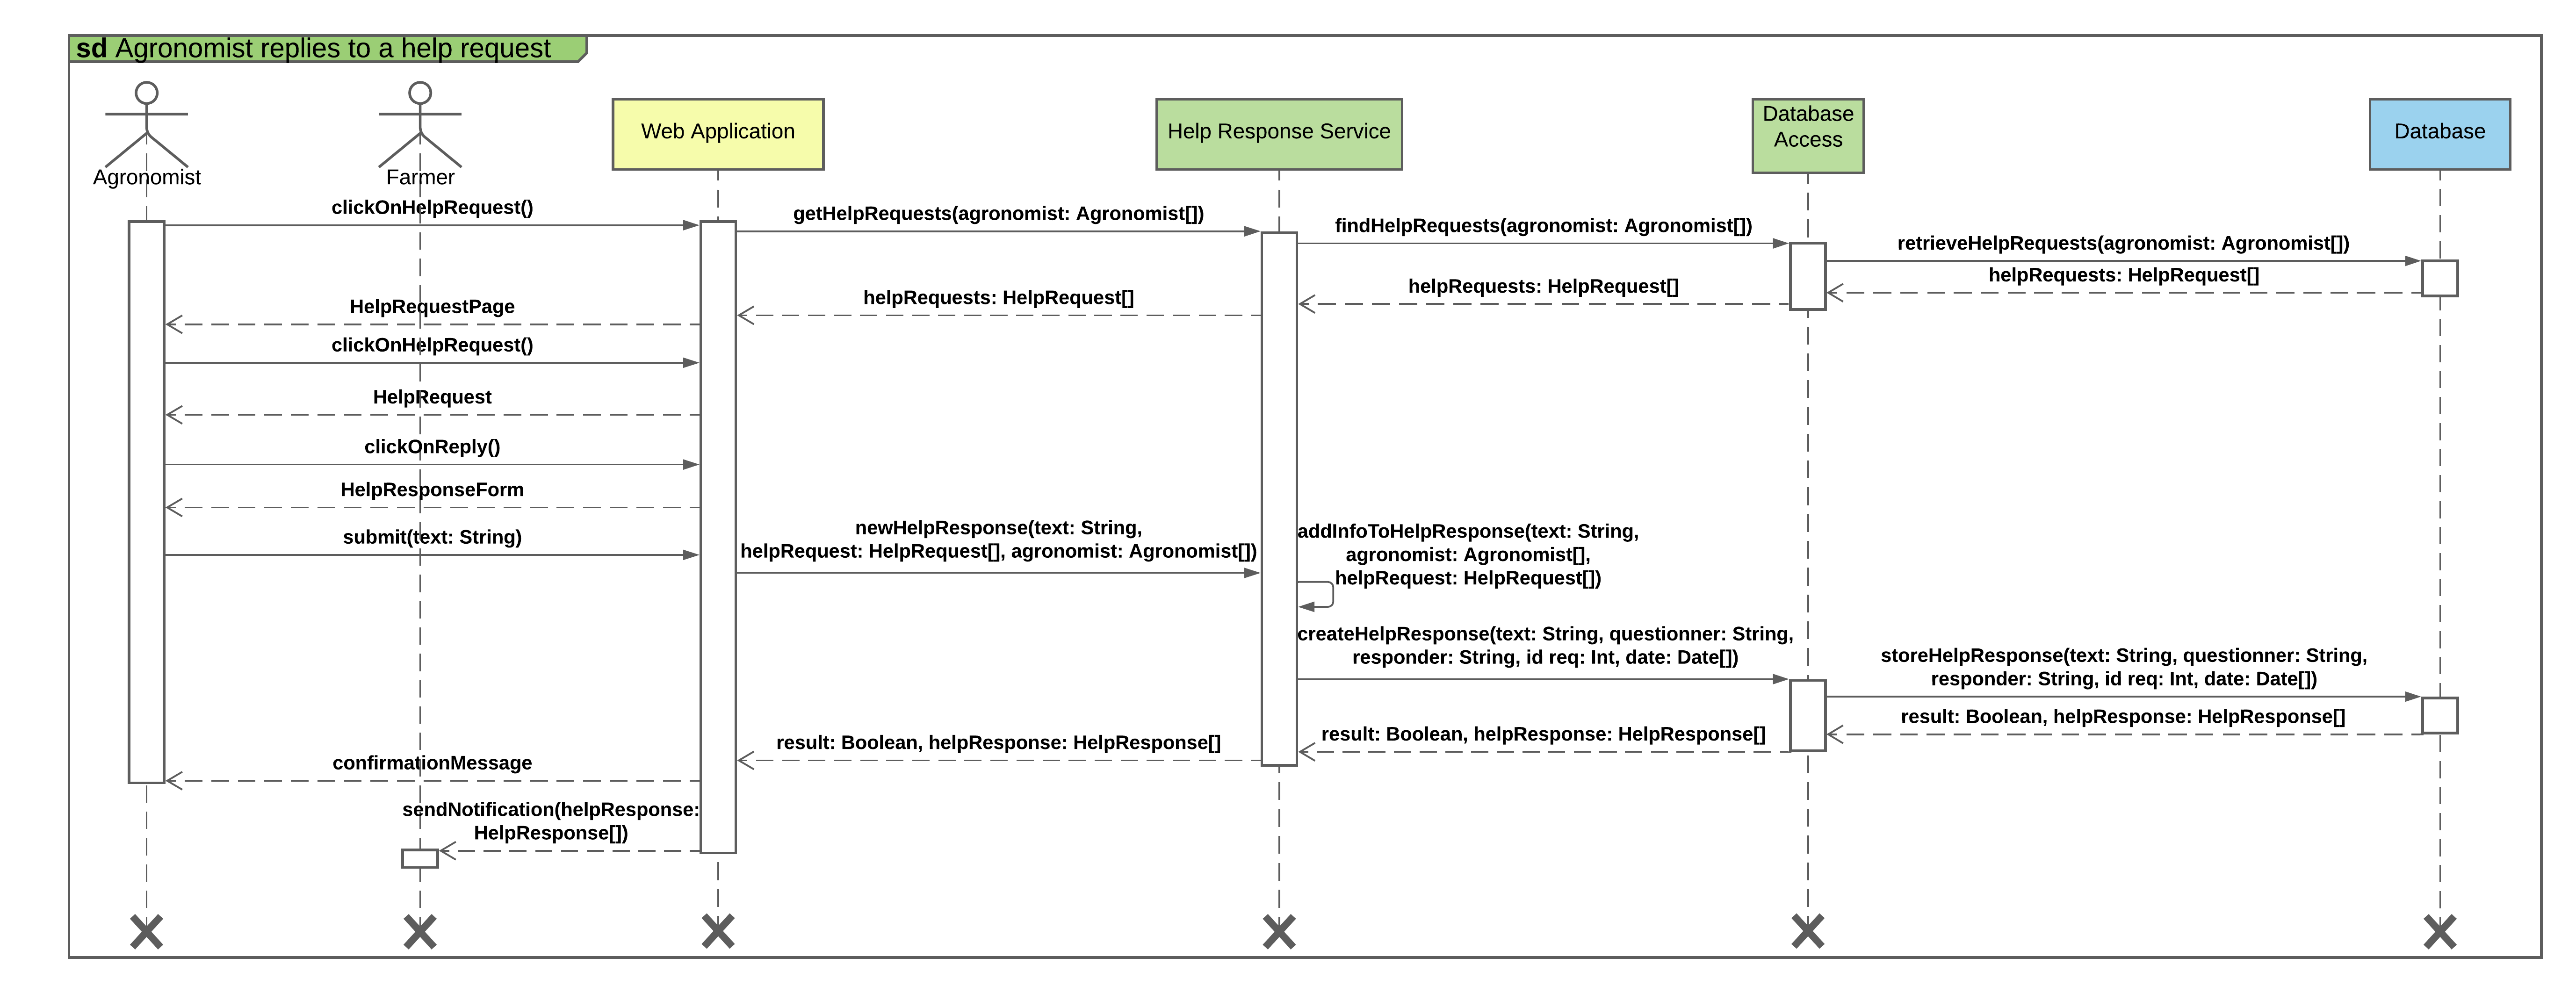
\includegraphics[scale= 0.108]{./Images/Sequence diagram/Agronomist replies to a help request.png}}
    \caption{Agronomist replies to a help request}
    \vspace*{-12cm}
\end{figure}
\fillandplacepagenumber
\end{landscape}

\subsection{Farmer solves a help request}

This sequence diagram shows the procedure of a farmer, already registered and logged in, solving a help request.\\
The farmer clicks on \textit{help request} icon. To return to the farmer the related page, Web/MobileApplication propagates a request to get all help requests and help responses related to the farmer to HelpRequestService which is able to retrieve them from the Database through DatabaseAccess. 
Once the \textit{help request} page is shown to the farmer, he/she clicks on \textit{my help requests} button to visualize those created by him/her and the related page is returned by Web/MobileApplication. The farmer solves a help request clicking on the related button and Web/MobileApplication calls a function to update the status of the help request. The request is propagated to HelpRequestService and then the help request state is updated in the Database. The result is returned to Web/MobileApplication following the same path. If result is false the operation must be repeated.

\newpage
\begin{landscape}
\begin{figure}[h]
\vspace*{-2cm}
\noindent
\centering
\centerline{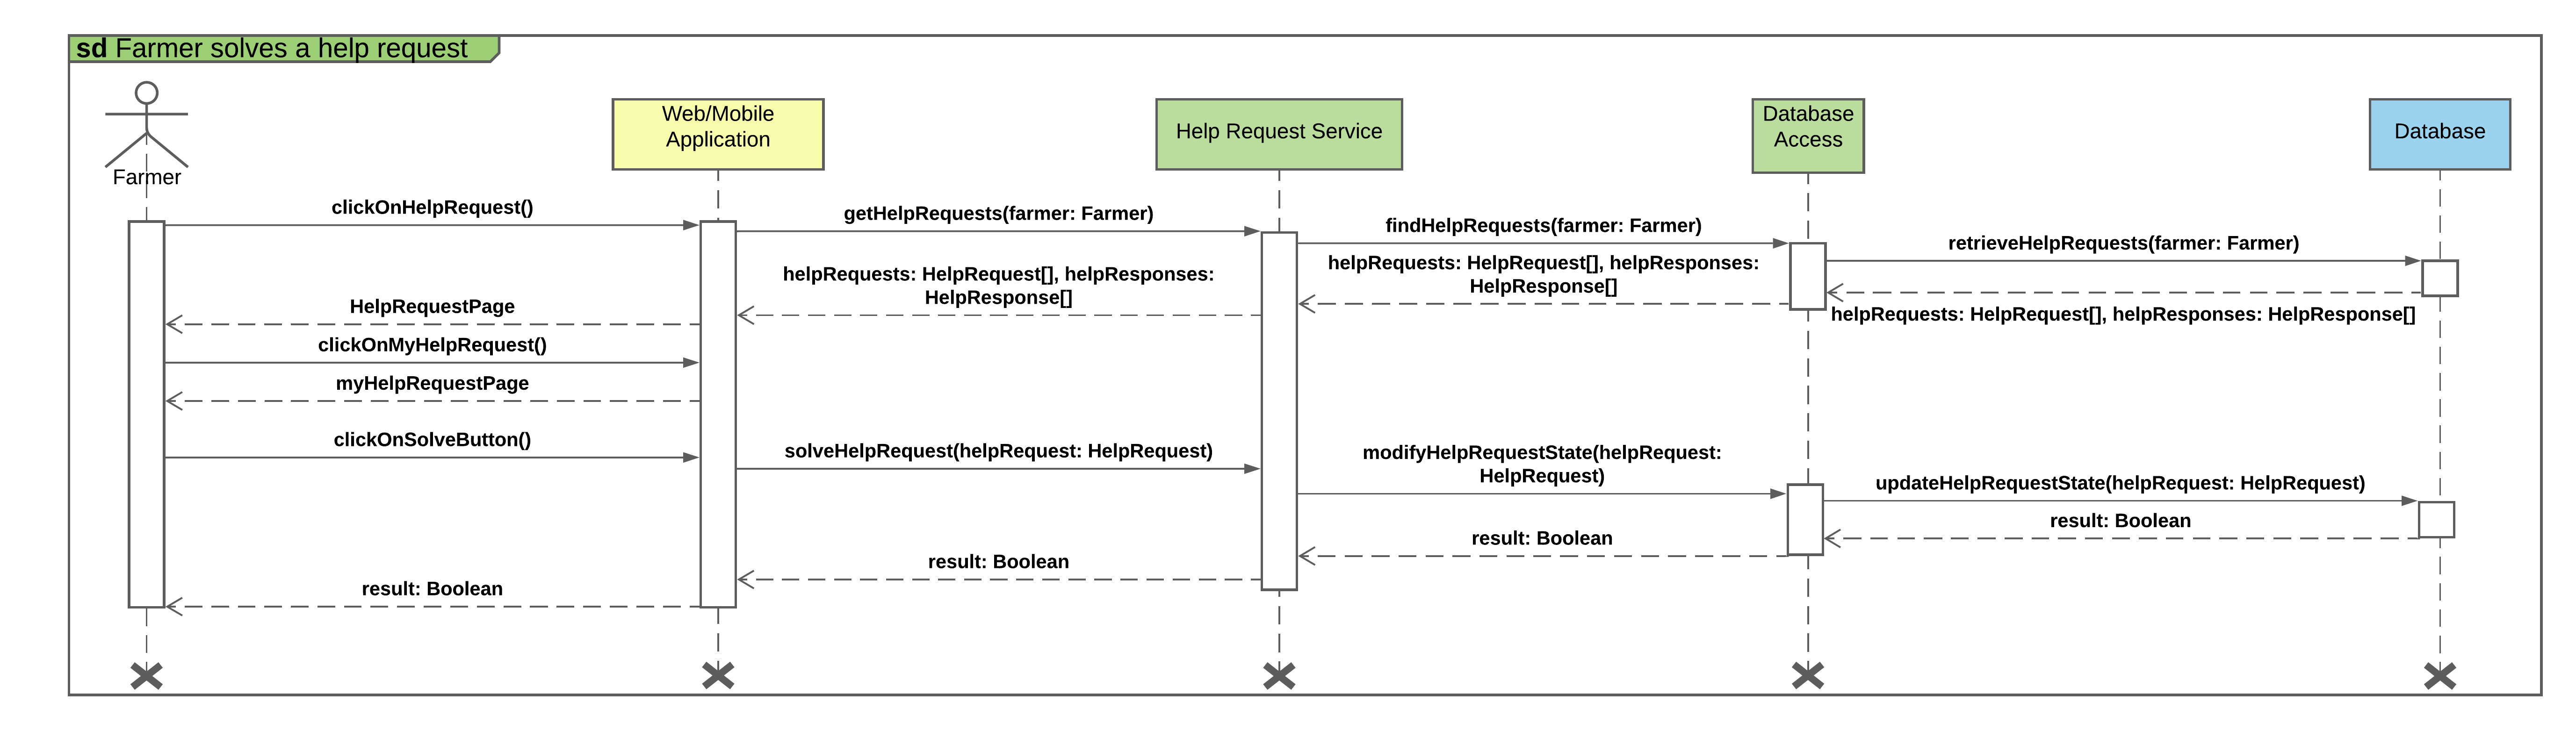
\includegraphics[scale= 0.108]{./Images/Sequence diagram/Farmer solves a help request.png}}
    \caption {Farmer solves a help request}
    \vspace*{-12cm}
\end{figure}
\fillandplacepagenumber
\end{landscape}

\subsection{Agronomist visualizes weather conditions}

This sequence diagram shows the procedure of an agronomist, already registered and logged in, visualizing weather conditions.\\
The agronomist clicks on \textit{weather} icon.
He/she can optionally select the date (from the current day up to seven day) for which he wants to visualize data. By default, if he/she doesn't select anything, the system shows him weather conditions for the current day. To return to the agronomist the related page, Web/MobileApplication propagates a request to get the weather map of his/her mandal to WeatherForecastsService which is able to retrieve weather and soil moisture data from external APIs (TelanganaGovernmentService and CopernicusClimateDataStoreService).
Then, data retrieved are returned to WeatherForecastsService which is in charge also of processing the mandal weather map interacting with GoogleMapsAPI.  
Eventually, the map is shown to the agronomist.

\newpage
\begin{landscape}
\begin{figure}[h]
\vspace*{-2cm}
\noindent
\centering
\centerline{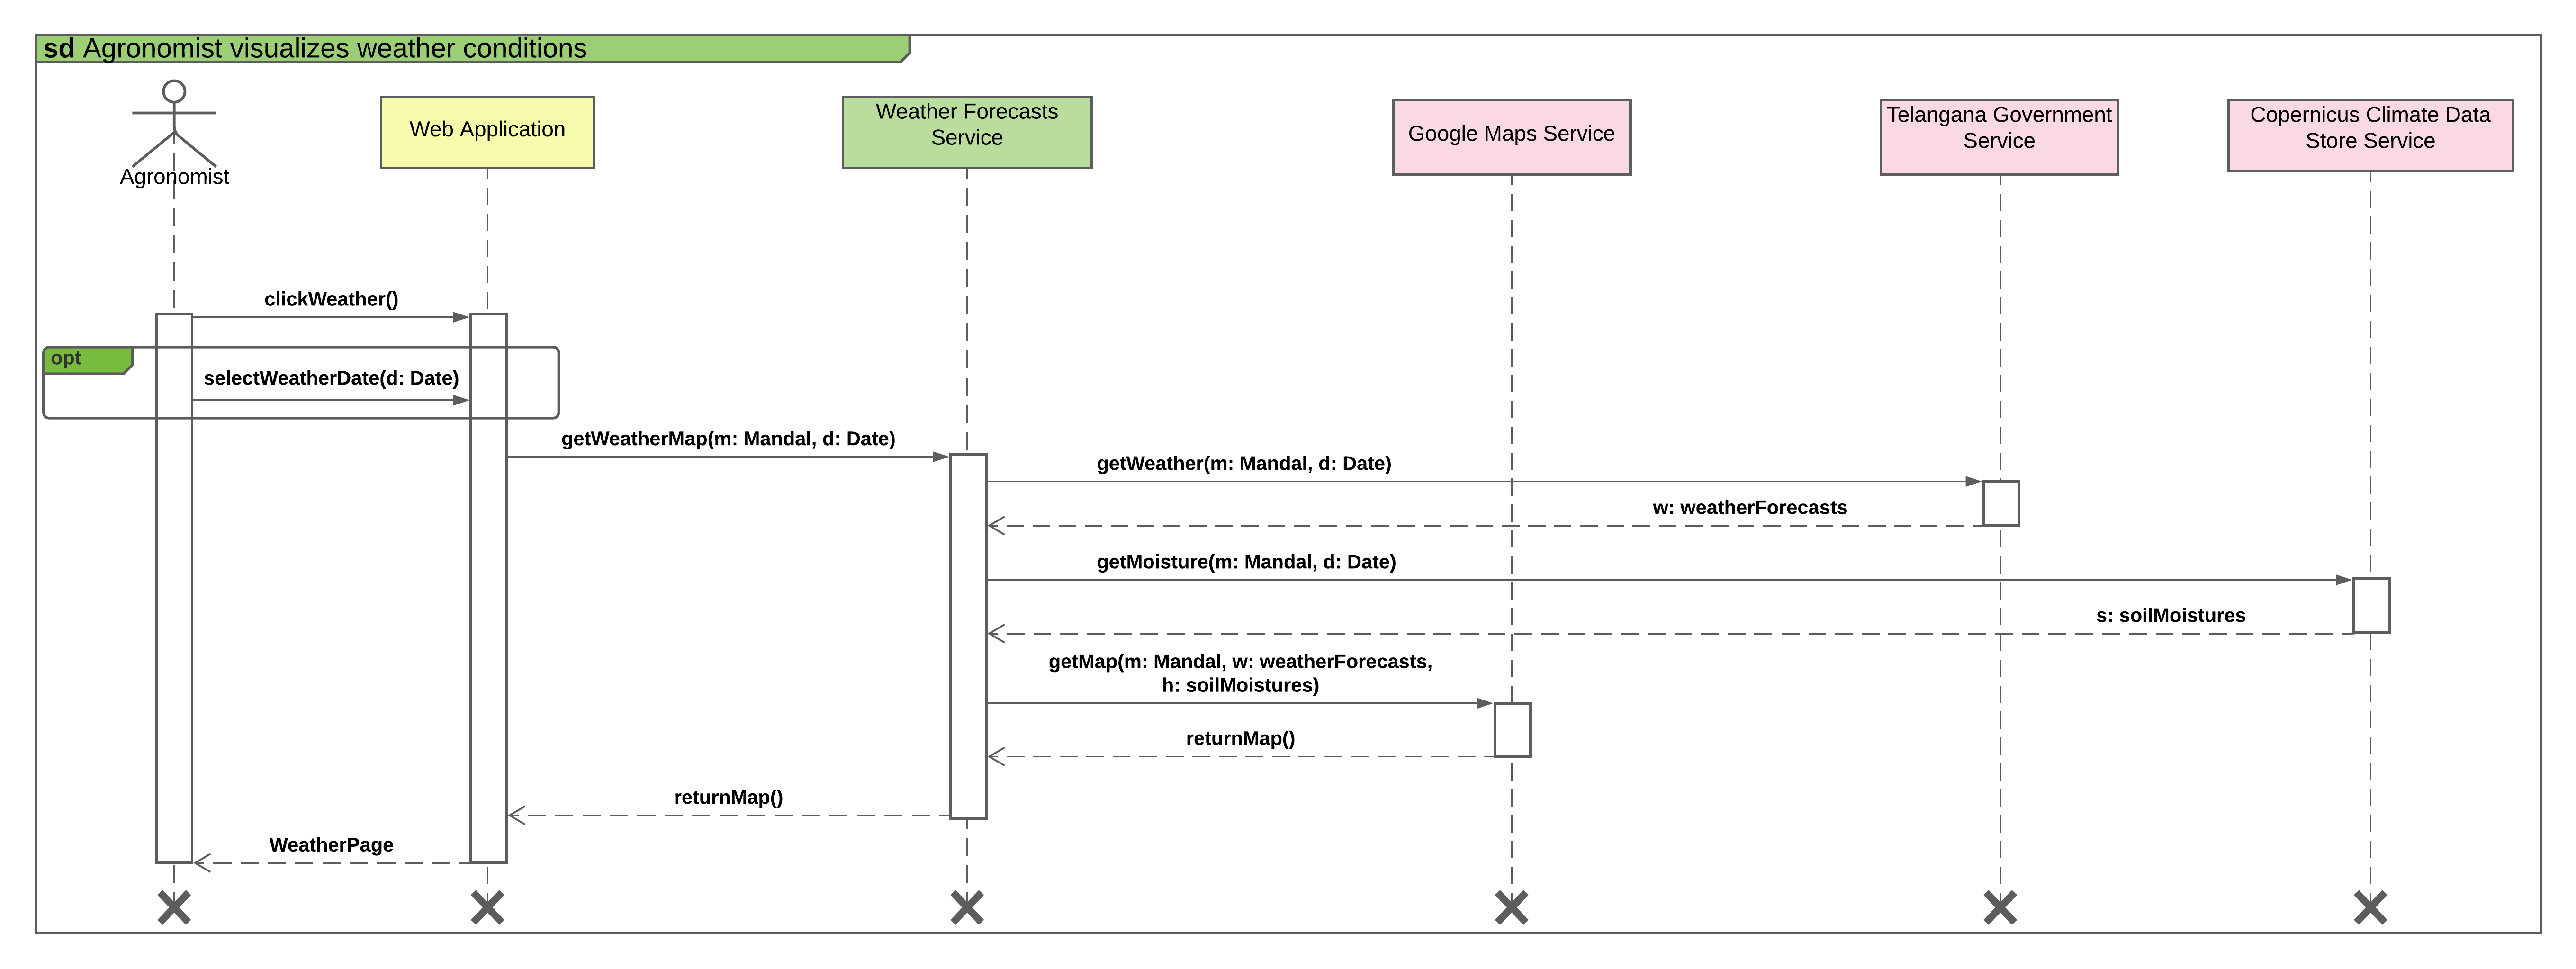
\includegraphics[scale= 0.108]{./Images/Sequence diagram/Agronomist visualizes weather conditions.png}}
    \caption{Agronomist visualizes weather conditions}
    \vspace*{-12cm}
\end{figure}
\fillandplacepagenumber
\end{landscape}

\subsection{Agronomist visualizes and analyzes farmers' data}

This sequence diagram shows the procedure of an agronomist, already registered and logged in, visualizing and analyzing his/her mandal's farmers' data in the homepage of the application.\\
The agronomist opens the application. 
Web/MobileApplication propagates two requests, one to TableService to get a table of farmers' performances in descending order and the other one to MandalMapService to get the mandal map on which are displayed farmers's performances scores. For both services is necessary to retrieve from the Database mandal's farmers' data (including performances and positions). Those data are returned to TableService and to MandalMapService. The latter component is in charge of processing the map to be displayed to the agronomist, for this reason it interacts with GoogleMapAPI external service.
Eventually the \textit{homepage} is shown to the agronomist.

\newpage
\begin{landscape}
\begin{figure}[h]
\vspace*{-2cm}
\noindent
\centering
\centerline{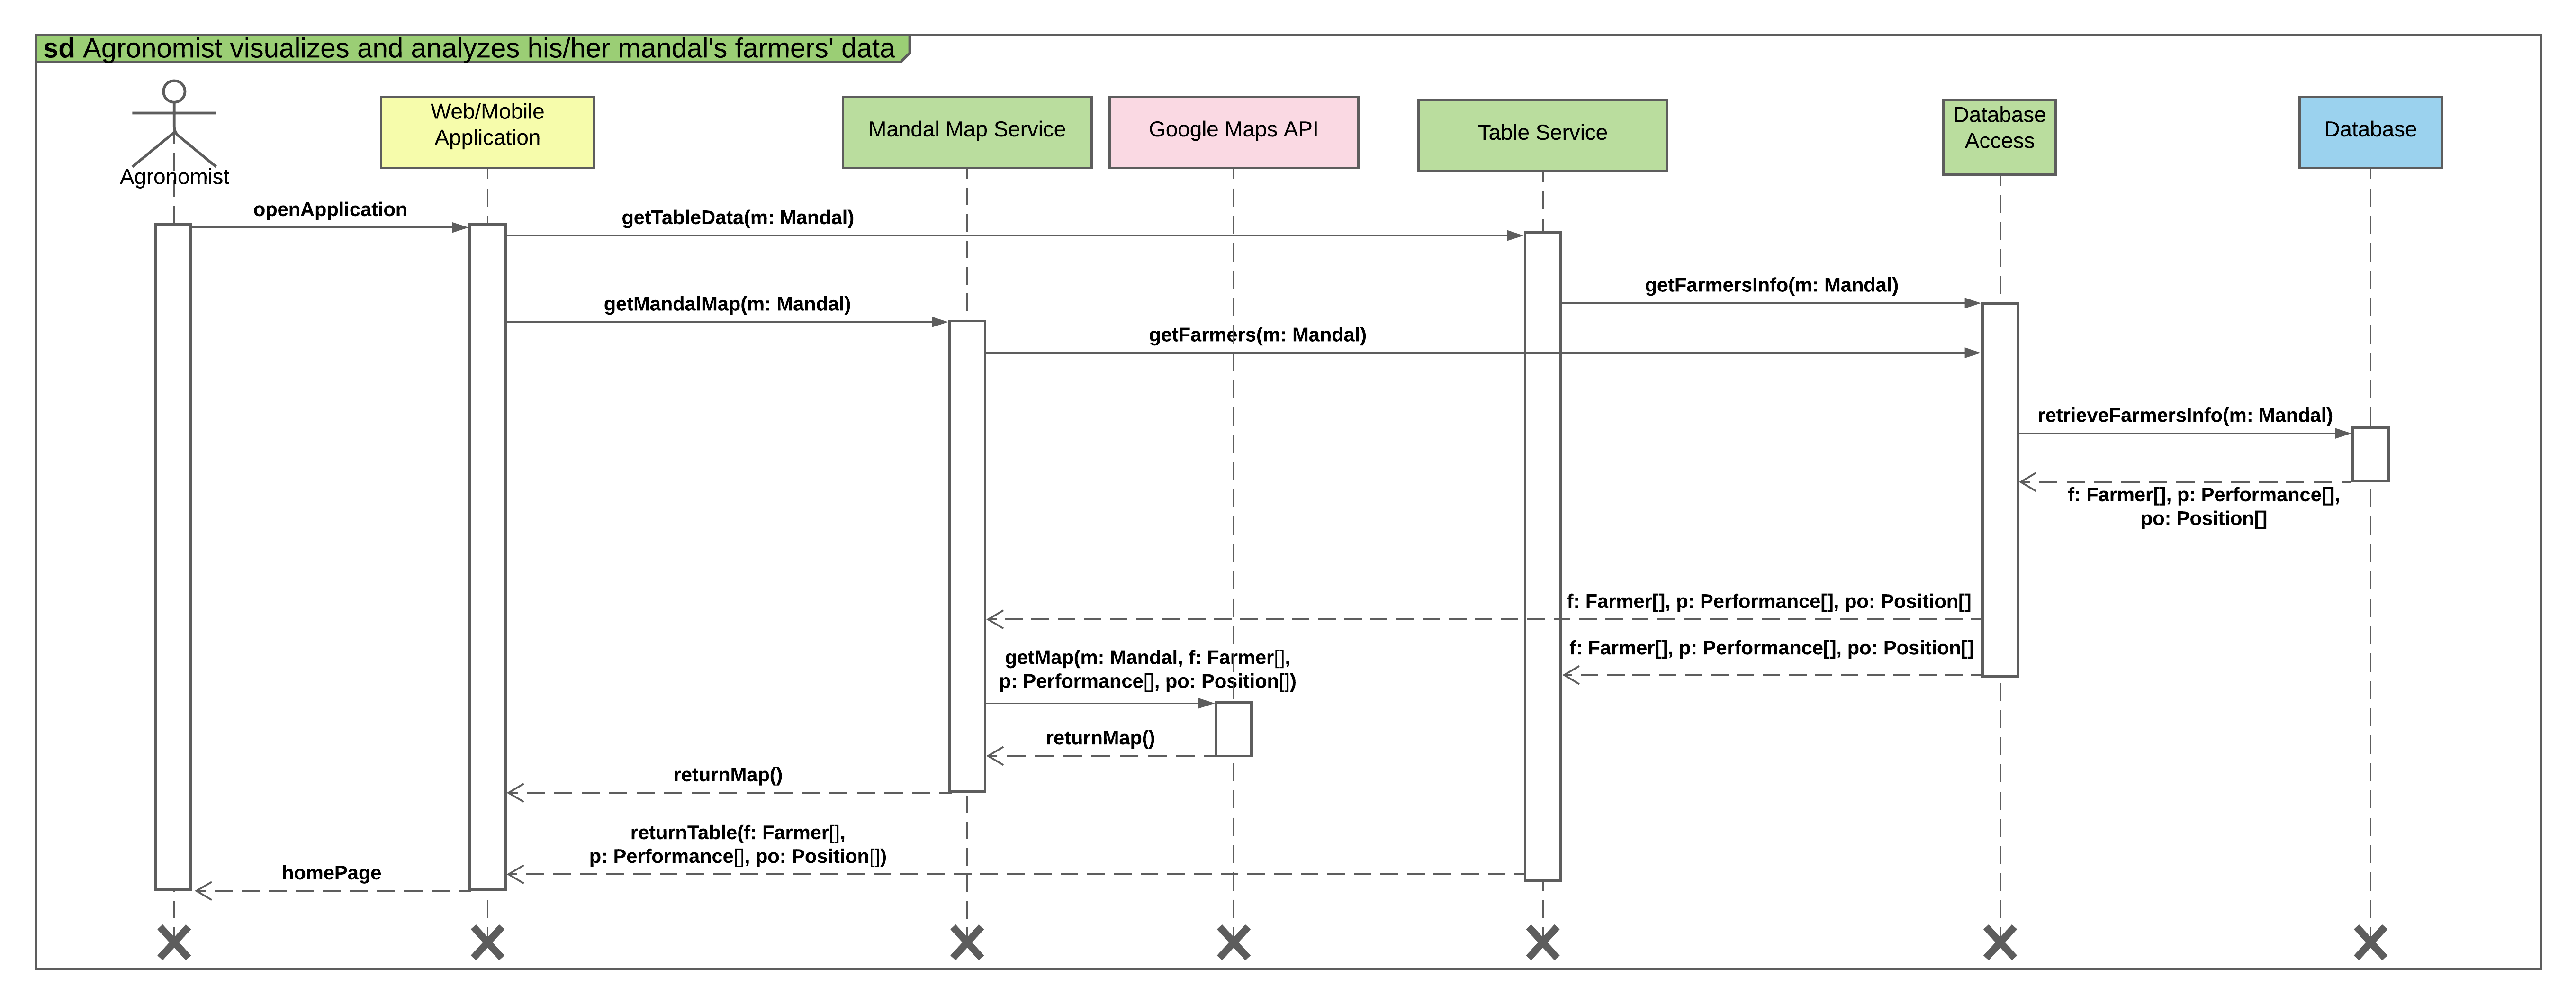
\includegraphics[scale= 0.108]{./Images/Sequence diagram/Agronomist visualizes and analyzes his_her mandal's farmers' data.png}}
    \caption{Agronomist visualizing and analyzing farmers' data Sequence Diagram}
    \vspace*{-12cm}
\end{figure}
\fillandplacepagenumber
\end{landscape}

\subsection{Agronomist updates his/her daily plan}

This sequence diagram shows the procedure of an agronomist, already registered and logged in, updating his/her daily plan.\\
The agronomist clicks on \textit{daily plan} icon. To return to the agronomist the related page, Web/MobileApplication propagates a request to get all daily plans and visits related to the agronomist to DailyPlanService which is able to retrieve them from the Database through DatabaseAccess. 
Once the \textit{daily plan} page is shown to the agronomist, he/she clicks on \textit{update} button. The update form is returned by Web/MobileApplication. The agronomist fills out the form and a function is called by Web/MobileApplication to get the visit corresponding to date and hour inserted by the agronomist. The function is propagated to DailyPlanService which is in charge of finding the visit and returns it following the same path. If result is false no visit was found and a new visit is created and stored in the Database. If result is true a visit with the date and hour inserted by the agronomist already exists, for this reason it is updated in the database according to the information entered by the user. In both cases, the visit's status is set into scheduled and the corresponding daily plan's state is change into updated. 
Eventually the result and the visit are returned following the same path and a notification is sent to the farmer whose visit has been created/changed.

\newpage
\begin{landscape}
\begin{figure}[h]
\vspace*{-2cm}
\noindent
\centering
\centerline{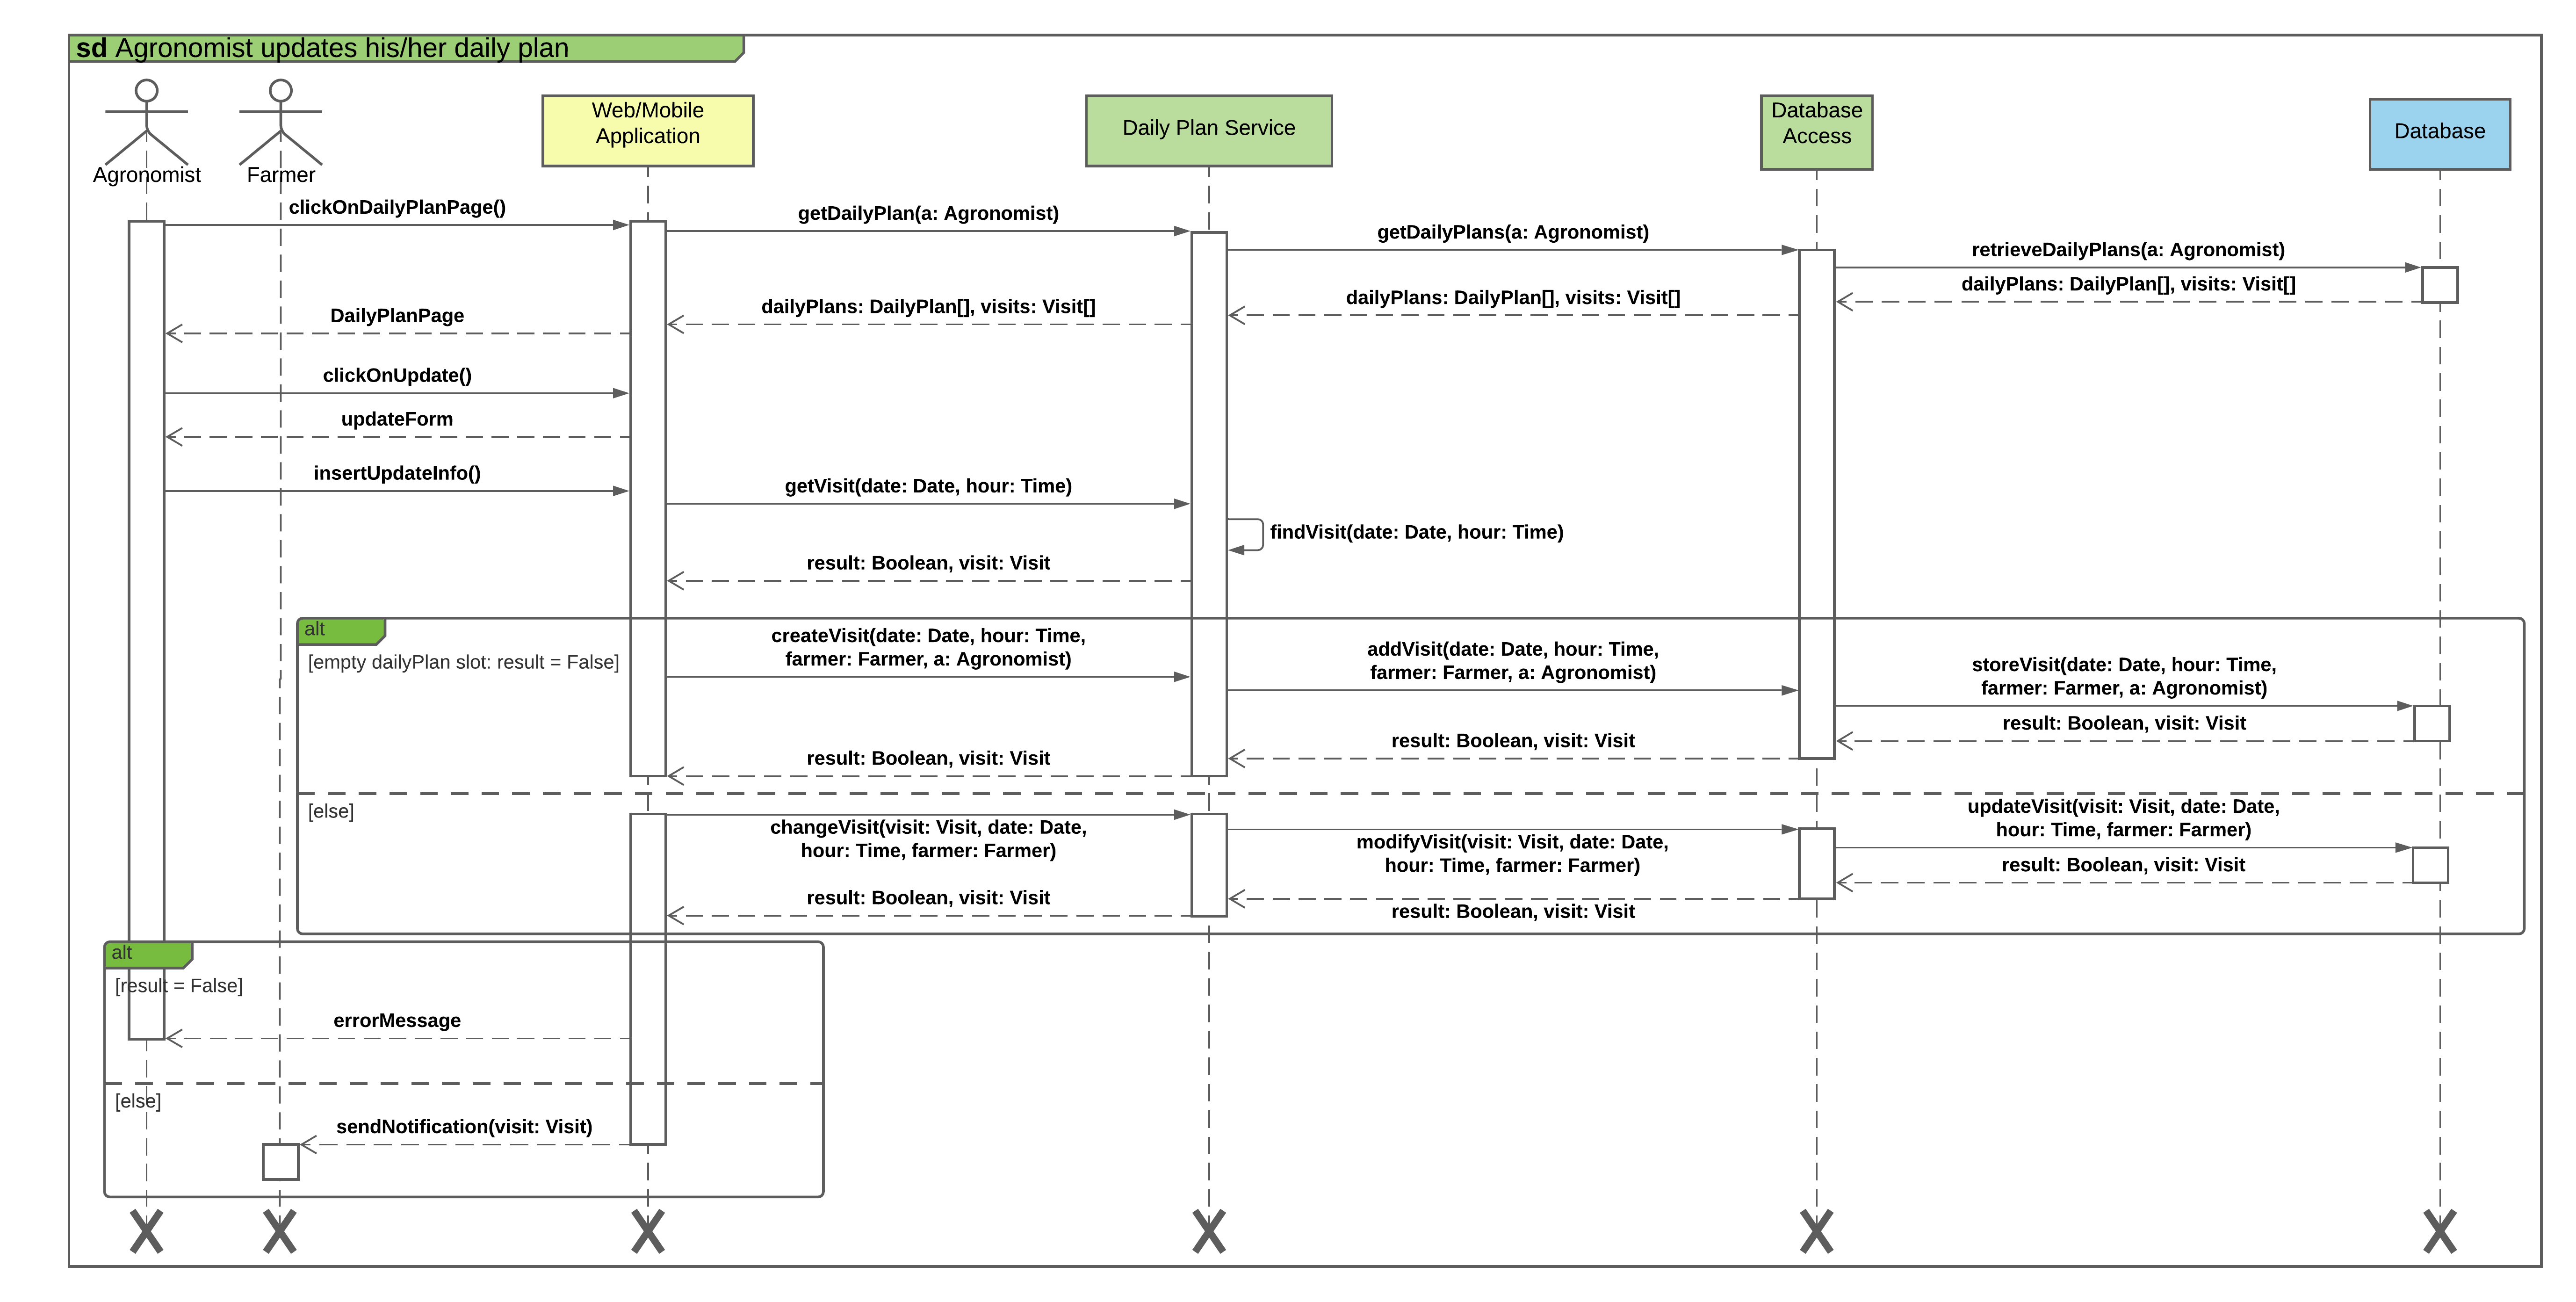
\includegraphics[scale= 0.108]{./Images/Sequence diagram/Agronomist updates his_her daily plan.png}}
    \caption{Agronomist updates his/her daily plan}
    \vspace*{-12cm}
\end{figure}
\fillandplacepagenumber
\end{landscape}


\subsection{Agronomist confirms his/her daily plan}

This sequence diagram shows the procedure of an agronomist, already registered and logged in, confirming his/her daily plan.\\
The agronomist clicks on \textit{daily plan} icon. To return to the agronomist the related page, Web/MobileApplication propagates a request to get all daily plans and visits related to the agronomist to DailyPlanService which is able to retrieve them from the Database through DatabaseAccess. 
Once the \textit{daily plan} page is shown to the agronomist, he/she clicks on a certain daily plan page and a function to retrieve the selected daily plan and related visits is called by Web/MobileApplication and propagated to DailyPlanService which is in charge of finding the selected daily plan. The result is returned following the same path and daily plan details are shown to the agronomist. He/she clicks on \textit{confirm} button and the confirmation form is returned by Web/MobileApplication. The agronomist optionally insert deviations from the daily plan in the appropriate field and then submits. Then, a function is called and propagated by Web/MobileApplication change the state of the daily plan into confirmed and related visits' status into done in the Database. 
Eventually the result is returned following the same path.
If result is false the process must be repeated. 

\newpage
\begin{landscape}
\begin{figure}[h]
\vspace*{-2cm}
\noindent
\centering
\centerline{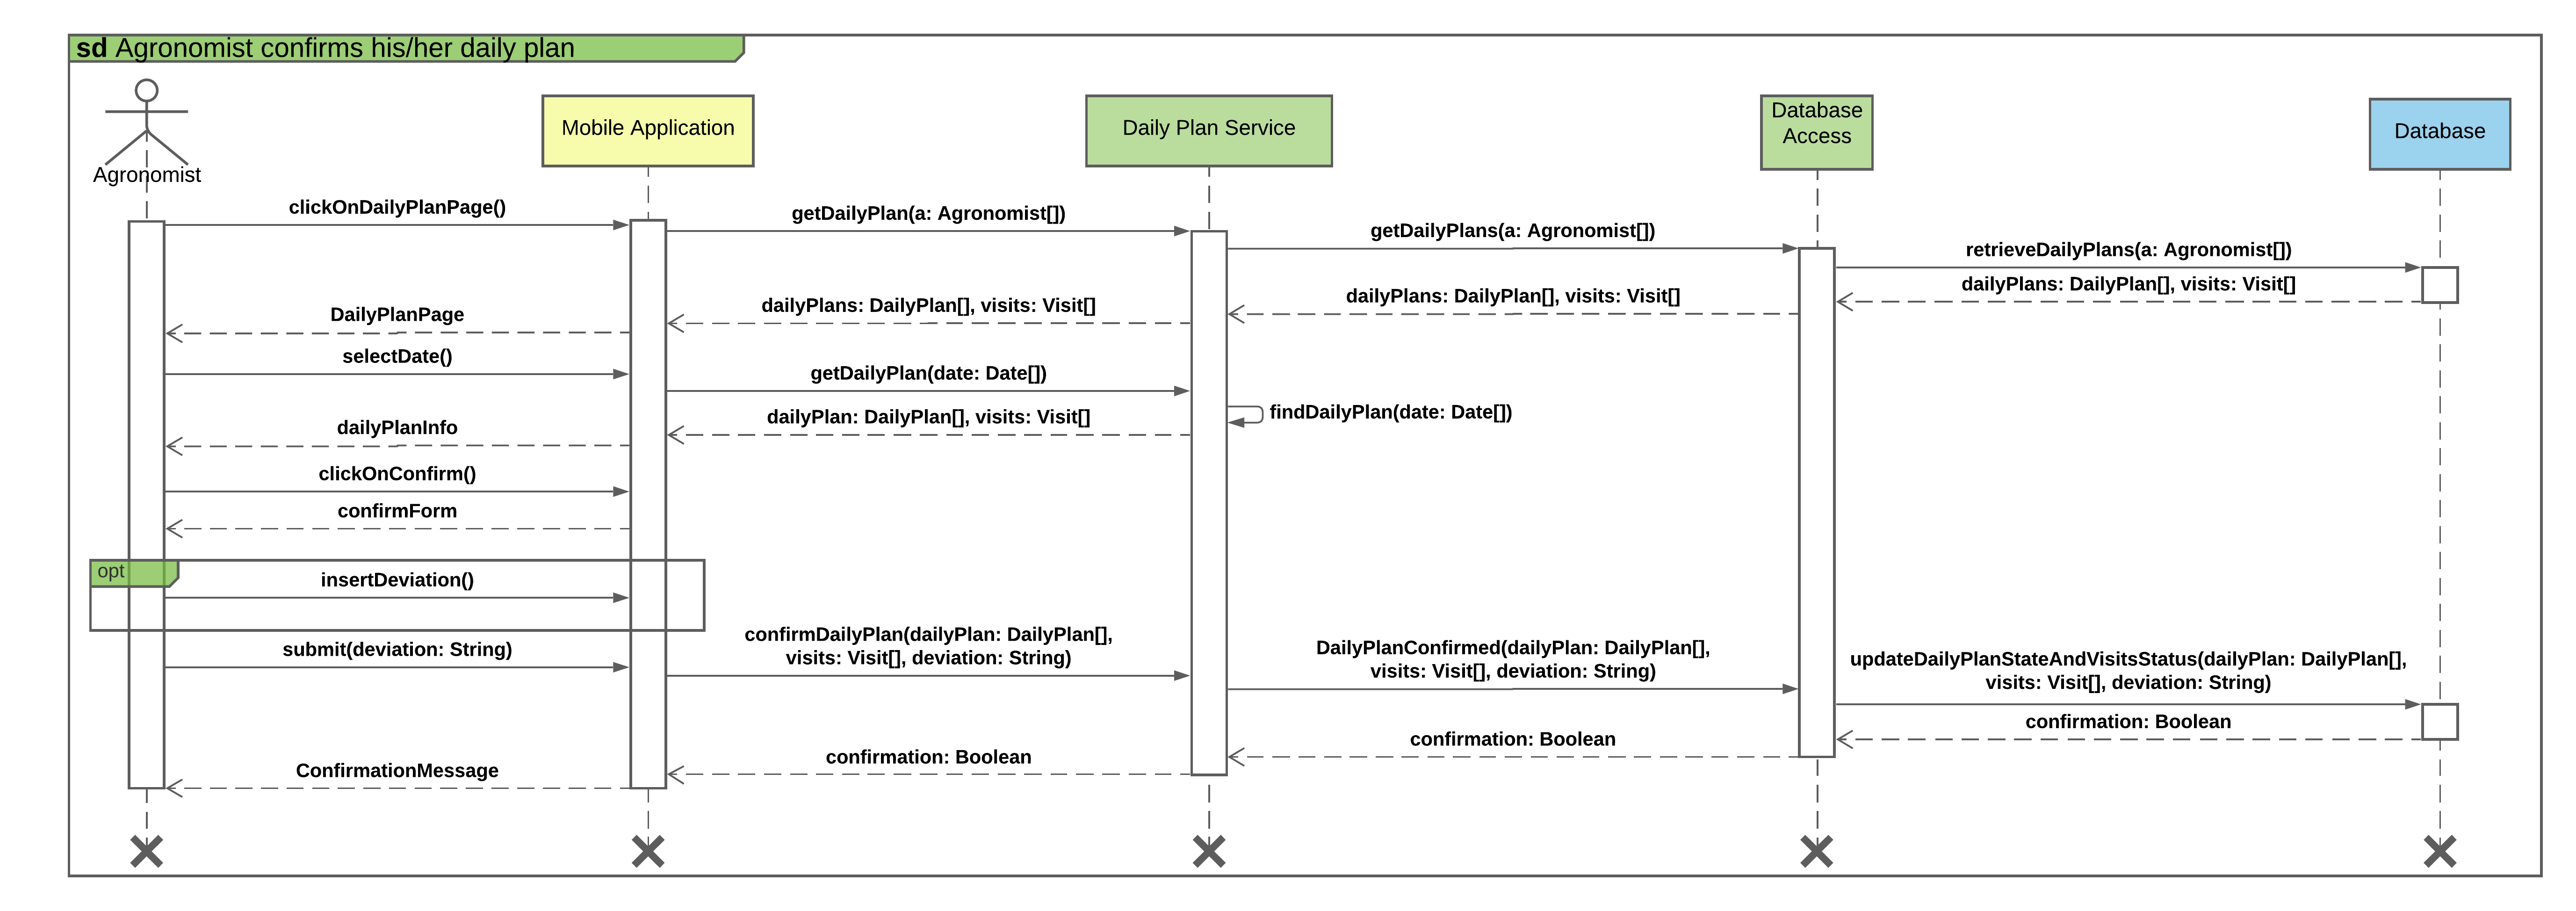
\includegraphics[scale= 0.108]{./Images/Sequence diagram/Agronomist confirms his_her daily plan.png}}
    \caption{Agronomist confirms his/her daily plan}
    \vspace*{-12cm}
\end{figure}
\fillandplacepagenumber
\end{landscape}

\subsection{Policy Maker visualizes and analyzes farmers' data}

This sequence diagram shows the procedure of a policy maker, already registered and logged in, visualizing and analyzing farmers' data in the homepage of the application.\\
The policy maker opens the application and he/she can select map and time chart options. If no option is modified the system process time chart and map automatically with default parameters.  
Web/MobileApplication propagates two requests, one to TimeChartService to get a chart of farmers' performances trend and the other one to MapService to get the Telangana map on which are displayed farmers's performances. For both services is necessary to retrieve from the Database farmers' data(performances and positions). Those data are returned to TimeChartService and to MapService. Both of them compute data according to the parameters selected by the policy maker or those acquired by default, then they return the result. In particular MapService is in charge of processing the map on which will be displayed farmers' performances, to do so it interacts with GoogleMapsAPI external service.
Eventually the \textit{homepage} is shown to the policy maker.

\newpage
\begin{landscape}
\begin{figure}[h]
\vspace*{-2cm}
\noindent
\centering
\centerline{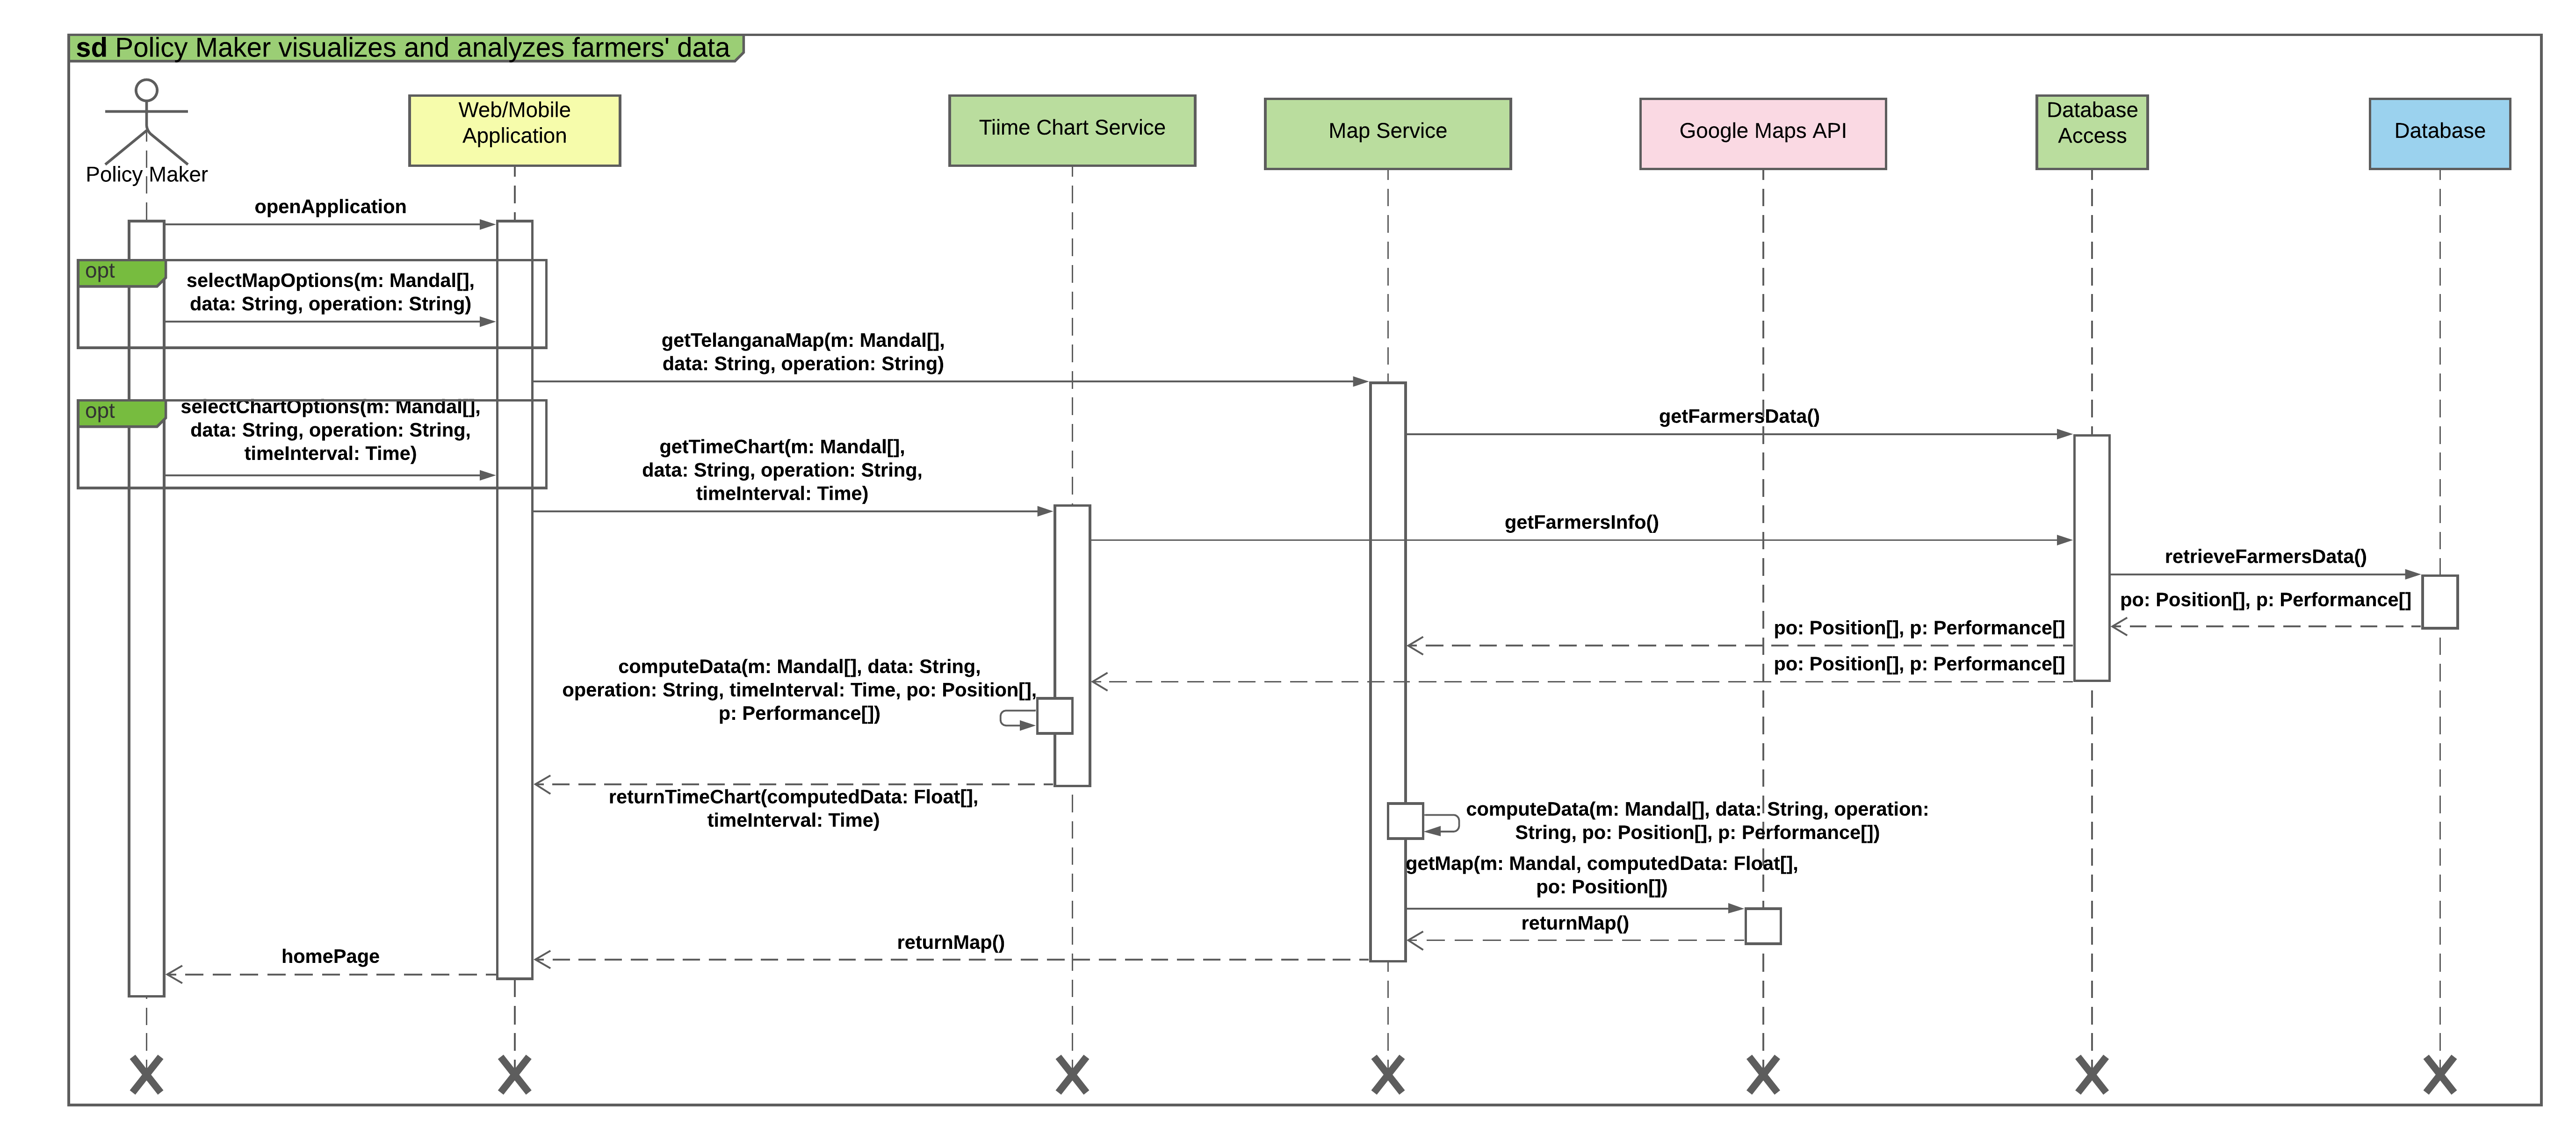
\includegraphics[scale= 0.108]{./Images/Sequence diagram/Policy Maker visualizes and analyzes farmers' data.png}}
    \caption{Policy Maker visualizes and analyzes farmers' data}
    \vspace*{-12cm}
\end{figure}
\fillandplacepagenumber
\end{landscape}

















